
\graphicspath{{part_5/figures}{part_5/figures/}}



In this chapter, we aim at extending the previous works to the control
synthesis of partial differential equations, mainly used to model mechanical systems. 
While the model of switched systems are usually used for (low dimensional)
ordinary differential equations controlled with a piecewise constant function,
it is also possible to use these models for control of mechanical systems. 
Indeed, the dynamics of most mechanical 
systems can be modeled by partial differential equations, and the spacial discretization
of such systems leads to high dimensional ODEs. Controlled with a piecewise constant function on
the boundary, and written in a proper way (the state space representation), 
one obtains high dimensional switched control systems.
As stated in Chapter \ref{chap:1}, the computational cost of the synthesis algorithms
is exponential in the dimension of the system.
Whether a finite element, a finite difference, or any discretization method is used,
an accurate discretized model of a mechanical system leads to ODEs of dimension
greater than $1000$. The dimension of real case studies used in industry 
often exceeds $10^6$. 
It is thus irrelevant to directly use the algorithms of Chapter \ref{chap:1} to
discretized PDEs. 
A model order reduction is required in order to synthesize a controller 
at the reduced-order level.
In this chapter, linear systems are considered, and we will use 
the reachability computations of Chapter~\ref{chap:1.1} since 
they provide the most accurate results. 
Two methods are propose: a fully offline procedure, and a semi-online procedure 
requiring online state estimation.
The state is first supposed known at every time, we then provide a first step
to the use of online state observers. 
Note that the synthesis is always performed offline, we refer to semi-online because the application
of the induced controller requires online state estimation.


% We focus here on switched control systems, a class of hybrid systems
% recently used with success in various domains such as automotive industry 
% and power electronics. 
% Several strategies have been developed to design control laws for 
% such systems; however the associated algorithms are very expensive and 
% require a limited state space dimension,
% Here, the invariance analysis \cite{FS-book13,FKS-safety,FS-rp13} is used to synthesize controllers, 
% an offline and an online procedure are proposed to apply the controller to the full-order system. 
% Offline and online controls are developed, and the computation of upper bounds of the 
% error induced by the reduction allows to guarantee the effectiveness of the controller.
% Note that this paper is an extension of the conference paper \cite{lecoent15}, it includes 
% some missing parts, more test cases, and the applications belong to the field of mechanics.


\vspace{1em}

{\bf Comparison with related work.}

Model order reduction techniques for hybrid or switched systems are classically used in
{\em numerical simulation}   in order to construct, at the reduced level,
trajectories  which cannot be computed directly at the original level
due to complexity and large size dimension \cite{Antoulas-Sorensen-Gugercin00,chinesta2011short}.
Model reduction is used in order to perform  
{\em set-based reachability analysis} in \cite{Han-Krogh04}.
Isolated trajectories issued from  isolated points are not constructed,
but  (an over-approximation of) the infinite set of trajectories
issued  from a dense set of initial points. This allows to perform formal verification
of properties such as {\em safety}. In both approaches, the control is {\em given}
as an input of the problem. 
In contrast here, the control is {\em synthesized} using set-based methods
in order to achieve by construction properties such as 
{\em convergence} and {\em stability}. 


While symbolic approaches are mostly used for the control of low order
ODEs, the control of mechanical systems can be realized using the control theory approach, 
where a continuous control law is guessed and proved to be efficient on the continuous
PDE model \cite{shahruz1998,azam1994nonlinear} {\todo et plein d'autres \cite{???}}. 
The damping of vibration with 
piezoelectric devices is in particular a widely developed branch of the control
of mechanical systems. The shunting of piezoelectric devices with
electric circuits permits to convert the vibration energy into electric energy,
which is then dissipated in the electric circuits \cite{hagood1991}.
Note that this approach can be active or passive, depending on the electric energy furnished
to the electric circuit.
A switched control approach is developed in \cite{clark2000vibration,ramaratnam2004semi}, 
the piezoelectric
device is shunted on several electric circuits, but only one is selected at a time depending
on the state of the mechanical system. This approach is called semi-active since the electric
circuits are passive but the switching requires energy.
In the present paper, the approach is fully active.

\vspace{1em}

{\bf Plan.}

In Section \ref{sec:background_part5}, we give some preliminaries
on switched control systems and their link with PDEs and mechanical systems.
In Section \ref{sec:control}, we introduce some elements of control theory and 
the state-space bisection method.
In Section \ref{sec:reduction}, we explain how to construct
a reduced model, apply the state-space bisection method at this level, and compute
upper bounds to the error induced at the original level.
In Section \ref{sec:ROC}, we propose two methods of control synthesis
allowing to synthesize (either offline or online) a controller at the reduced-order level and apply it
to the full-order system.
In Section \ref{sec:examples}, we apply our approach to several examples of
the literature.
In section \ref{sec:observation}, we extend our method to the use of observers.
We conclude in Section \ref{sec:conclusion}.


\section{Background}\label{sec:background_part5}

We consider systems governed by Partial Differential Equations (PDEs) having actuators 
allowing to impose forces on the boundary; these systems can represent transient 
thermal problems, vibration problems...
By applying the right external force at the right time,
one can drive the system to a desired operating mode. Our goal here is 
to synthesize a law which, given the state of the system, computes the boundary force to apply.

In order to illustrate our approach, we use the example of the
heat equation:
\begin{equation} \left\lbrace
\begin{array}{ll}
  \dfrac{\partial T}{\partial t}(x,t) - \alpha \Delta T(x,t) = 0 & \forall (t,x) \in \lbrack 0,T \rbrack \times \Omega \\
  T(x,\cdot) = T^d(x,\cdot) & \forall x \in \partial \Omega^T \\
  \dfrac{\partial T}{\partial x}(x,\cdot) .n = \varphi^d(x,\cdot) & \forall x \in \partial\Omega^\varphi \\
  T(x,0) = T_0(x)
\end{array} \right.
\label{eq:heat_eq}
\end{equation}

Discretized by finite elements, the nodal temperatures $\{ T \}$ are computed
with respect to time, and the system becomes:
\begin{equation} \left \lbrace
\begin{array}{l}
 C_{FE} \dot{ \{ T \} } + K_{FE} \{ T \} = \{ F^d \} \\
\{ T(0) \} = \{ T_0 \}
 \end{array} \right.
 \label{eq:heat_eq_ef}
\end{equation}
The purpose is then to compute the forces $\{ F^d \}$ with respect to time such that
the temperature field verifies some desired properties.

For example, one may want to impose that the temperature in a particular node 
stays within a given temperature range. Usually, the quantities of interest one wants to 
control are given in discrete points, which are for example sensor 
measurements, or they are given as local averaging. Here, we consider
the case where the quantities of interest can be directly extracted from
the nodal values with a matrix called {\em output matrix} (see equation (\ref{eq:LTI})).

We consider a particular kind of actuators; the force applied only takes a finite number $N$ of values.
For example, in equation (\ref{eq:heat_eq}) for the case of a room heated with a heater, 
the flux $\varphi^d$ is equal to $0$ when the heater is turned off and 
equal to a positive value when it is turned on. The control systems associated to 
such behaviors are naturally written under the form of {switched systems}   \label{eq:switched_system0}.
% , and this is exactly the framework
% we place ourselves in.
% In control theory, such dynamical systems are written under the following form, called 
% {\em state-space representation}:
Focusing on linear PDEs, the addition of an output leads leads to a system of the form:
\begin{equation}
 \Sigma : \left\lbrace
\begin{array}{ll}
\dot x(t) & = A x(t)+B u(t), \\
 y(t) & =C x(t),
\end{array}
\right.
\label{eq:LTI}
\end{equation}
The $n$-vector $x$ is called the state of the system, the $p$-vector $u$ is the control
input, the $m$-vector $y$ is the output of the system,
$A$ is an $n\times n$-matrix, $B$ an $n\times p$-matrix, and
$C$ an $m\times n$ matrix. 
Writing the discretized equation (\ref{eq:heat_eq_ef}) under this form is straightforward 
by multiplying the first line by $C_{FE}^{-1}$ (which is invertible), and the state 
vector is then $\{T\}$. In the case of higher 
order PDEs (for example in the case of the wave equation), we merely need to enlarge the state vector
to take the first derivative of the nodal values in it.



\section{Problem setting}
\label{sec:control}


We will synthesize controllers using adaptations of
Algorithms \ref{algo:decomposition} and \ref{algo:findpattern}
by adding constraints on the outputs of the system. 

% An algorithm of control synthesis for switched control systems has been developed in
% % at the LSV laboratory at ENS Cachan 
% \cite{FKS-safety,FS-rp13}. This algorithm, called
% {\em state-space decomposition algorithm},
% allows the computation of control laws for low dimensional Ordinary Differential Equations.
% 
% In order to use this algorithm for the control of high dimensional discretized PDEs, we first 
% give some preliminary notions and results of control theory. 

% \subsection{Preliminaries}
% 
% As we place ourselves in the framework of switched control systems,
% the control variable $u$ of a given system $\Sigma$ takes 
% its values in a finite set $U$. The elements of $U$ are called the {\em switching modes}.
% The algorithm developed allows to compute a law $u(x)$ that 
% permits to verify some desired properties. This means that,
% knowing the state $x$ of the system, one knows the switching mode to apply in
% order to verify the given properties. Such a law is thus called {\em state-dependent}.
% Note that the switching modes are applied during a time $\tau$, and thus 
% the law $u(x)$ gives the switching modes to apply at the times $k \tau$ with $k \in \mathbb{N}$.
% The type of control law we want to apply can be schematized in Figure \ref{fig:fig1}.
% \begin{figure}[ht]
% \centering
%  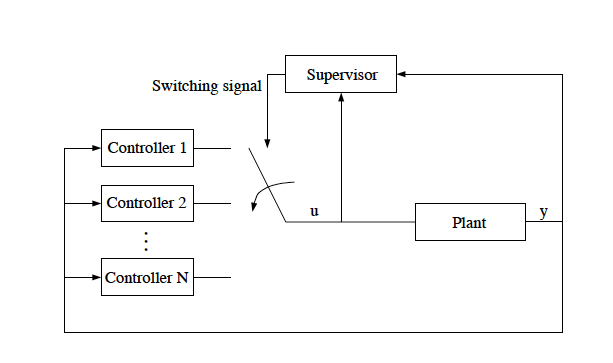
\includegraphics[width=84mm]{fig1.png}
%  \caption{Scheme of a switched control system}
%   \label{fig:fig1}
% \end{figure}



The entries of the problem are the following:
\begin{enumerate}
 \item a subset $R_x \subset \mathbb{R}^n$ of the state space, called {\em interest set},
 \item a subset $R_y \subset \mathbb{R}^m$ of the output space, called {\em objective set}.
\end{enumerate}
The objective is to find a law $u(\cdot)$ which, for any initial state $x_0 \in R_x$, 
stabilizes the output~$y$ in the set $R_y$. 
The set $R_x$ is in fact the set of all the initial 
conditions considered, and the set $R_y$ is a target set, where we want the output to stabilize.
The sets $R_x$ and $R_y$ are given under the form of boxes, i.e. interval products of
$\mathbb{R}^n$ and $\mathbb{R}^m$ respectively.

% We now introduce some notations and definitions required to present the algorithm.
%  We will
% use ${\bf x}(t,x,u)$ to denote the point reached by $\Sigma$ at time
% $t$ under switching mode $u\in U$ from the initial condition $x$.
% %
% This gives a  transition relation $\rightarrow_u^{\tau}$ defined for $x$ and $x'$ in $\mathbb{R}^n$ by:
% $x\rightarrow_u^{\tau} x' \mbox{ iff } \mathbf{x}(\tau,x,u)=x'$.
% %
% Given a set $X\subset\mathbb{R}^n$, we define the {\em successor set}
% of a set $X\subset \mathbb{R}^{n}$ of states under switching mode $u$ as:
% \[Post_u(X)=\{x' \ |\ x\rightarrow_u^{\tau} x'  \mbox{ for some $x\in X$}\}.\]
% As the systems considered are linear, 
% the set $Post_u(X)$ is the result of the affine transformation
% $A_dX + B_du$, where 
% $A_d = e^{A \tau}, \quad B_d = \int_0^{\tau} e^{A (\tau -t)}B dt$.

In the rest of this chapter, we will denote control patterns by $Pat \in U^k$
for some $k \geq 1$ in order to avoid confusion with projectors, classically denoted by $\pi$.
We extend the definition of the Post operator for outputs as follows:
the {\em output successor set} of a set $X\subset \mathbb{R}^{n}$
of states under switching mode $u$ is:
$$Post_{u,C} (X) = \bigcup_{x_0 \in X} C \phi_u(t; t_0, x_0).$$
% \[Post_{u,C}(X)=  \{Cx' \ |\ x\rightarrow_u^{\tau} x'  \mbox{ for some $x\in X$}\}.\]
We similarly extend this definition for sequences of inputs (patterns) 
$Pat \in U^k$ for some $k \geq 1$:
$$Post_{Pat,C} (X) = \bigcup_{x_0 \in X} C \phi_{Pat}(t; t_0, x_0).$$

% An {\em input pattern} named $Pat$ is defined as a finite sequence of switching modes. A 
% {\em $k$-pattern} is an input pattern of length at most $k$.
% The successor set of $X\subset \mathbb{R}^{n}$ using $Pat\equiv (u_1\cdots u_k)$ is defined by
% \[Post_{Pat}(X)=\{x' \ |\ x\rightarrow_{u_1}^{\tau}\cdots\rightarrow_{u_k}^{\tau} x',\ x\in X\}.\]
% The mapping $Post_{Pat}$ is itself an affine transformation. The output successor
% set of $X\subset \mathbb{R}^{n}$ using $Pat\equiv (u_1\cdots u_k)$ is defined by
% \[Post_{Pat,C}(X)=\{Cx' \ |\ x\rightarrow_{u_1}^{\tau}\cdots\rightarrow_{u_k}^{\tau} x',\ x\in X\}.\]

% 
% \subsection{State-Space Decomposition Algorithm}\label{sec:ssda}

With these definitions and notations, we are now able to present the adaptations of 
the algorithms presented in Chapter \ref{chap:0}. It relies on the decomposition
of the set $R_x$.  Given the sets $R_x$ and $R_y$, and a maximum length of 
input pattern $K$, it returns a set $\Delta$ 
of the form $\{(V_i,Pat_i)\}_{i\in I}$ where $I$ is a finite set of indexes. Every $V_i$
is a subset of $R_x$ and every $Pat_i$ is a pattern of length at most $K$, such that:
\begin{itemize}
\item[(a)] $\bigcup_{i \in I}V_i = R_x$,
\item[(b)] for all $i \in I$: $Post_{Pat_i}(V_i) \subseteq R_x$,
\item[(c)] for all $i \in I$: $Post_{Pat_i,C}(V_i) \subseteq R_y$.
\end{itemize}
{\todo est-ce qu'il faut laisser tout le  blabla suivant? pas trop r\'ep\'etitif avec le chapitre 1?} 

The algorithm thus returns several sets $V_i$ that cover $R_x$, and 
every $V_i$ is associated to a pattern $Pat_i$ that sends $V_i$ in $R_x$, and the output in $R_y$.
The set $R_x$ is thus decomposed in several sets, and for each one, we have 
one control law: $\forall x \in V_i, u(x) = Pat_i$. Therefore, for two 
initial conditions in a set $V_i$, we apply the same input pattern.
The fact that we use set based operations has a key role which allows us to consider 
sets of initial conditions, and this is how we manage to obtain
a law $u(x)$. In the following, when a decomposition $\Delta$ is successfully obtained , we denote
by $u_{\Delta}$ the induced control law.


% \begin{figure}[ht]
%  \centering
%  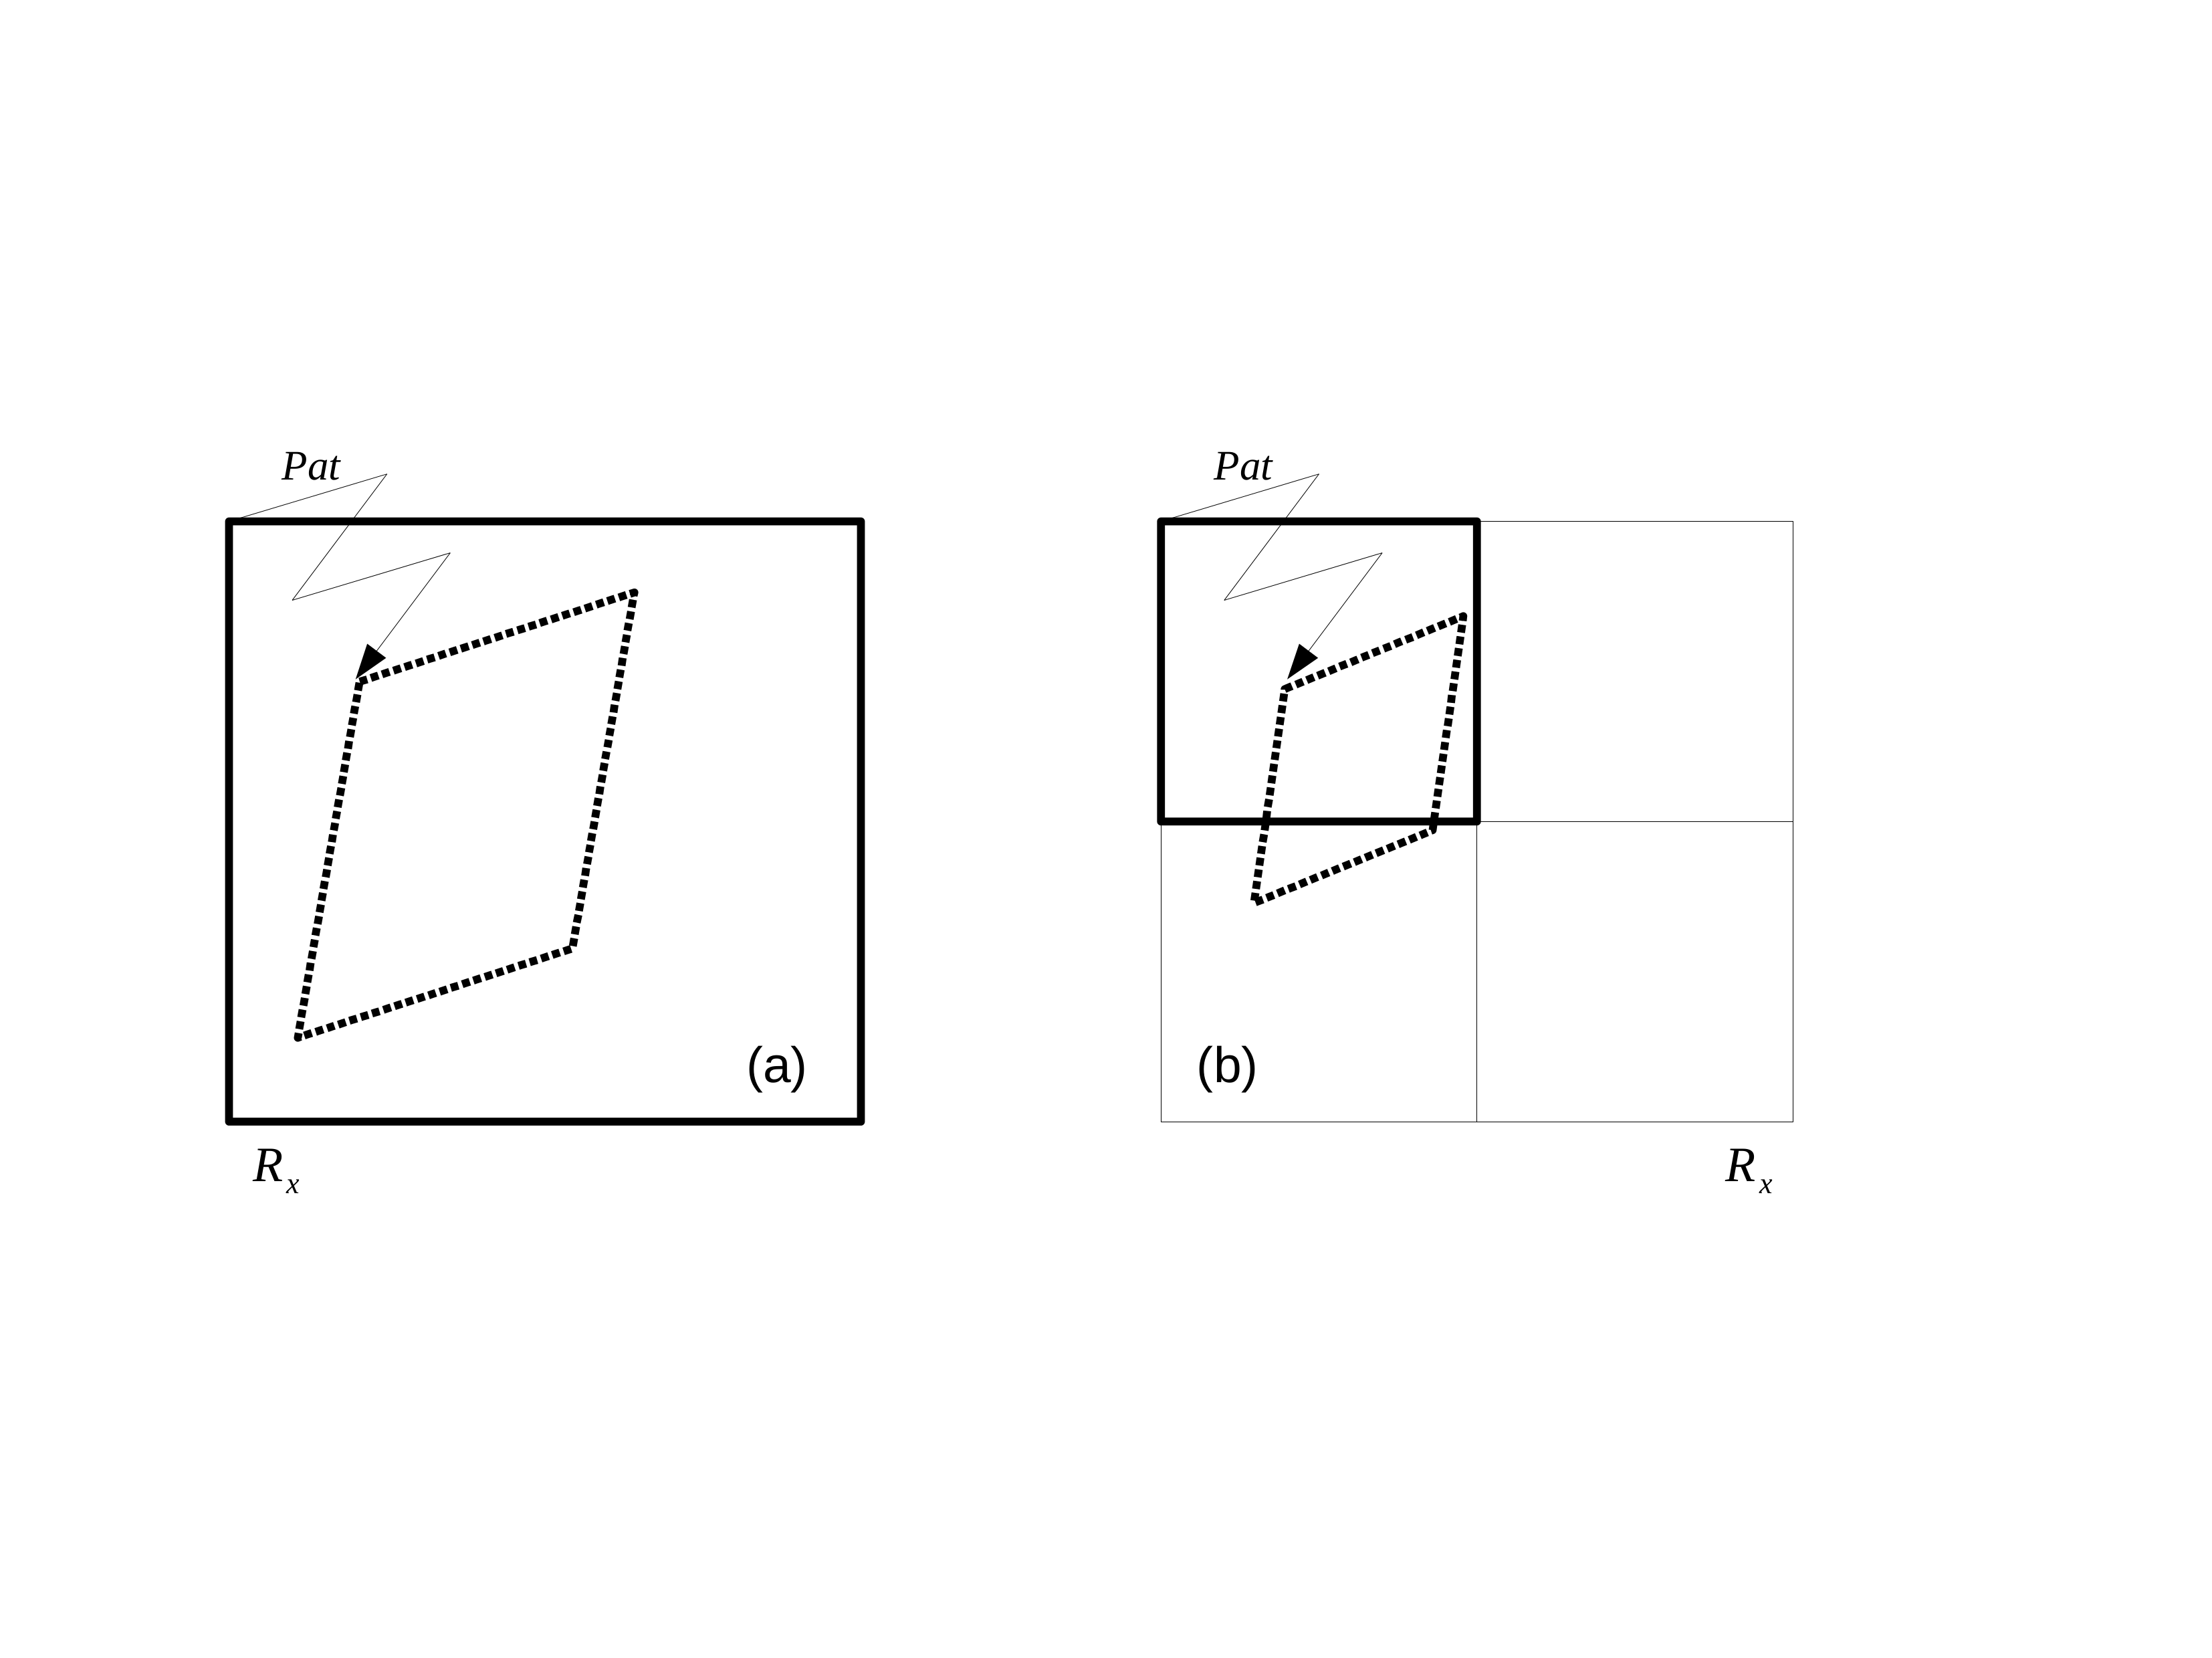
\includegraphics[trim = 2cm 5.5cm 5cm 5cm, clip, width=84mm]{fig2.png}
%  \caption{Scheme of the bisection algorithm. The real boxes are hypercubes in $n$ dimensions, they are
%  represented here by rectangles.}
%  \label{fig:fig2}
% \end{figure}
% 
% 
% The idea of the algorithm is the following: if we have an initial nodal vector $\{ T \}$ belonging 
% to a set $R_x = \lbrack T_{min},T_{max} \rbrack^n$, we want to apply a
% pattern that keeps $\{ T \}$ in $R_x$: the nodal temperatures, after application
% of the pattern, will still belong to $R_x = \lbrack T_{min},T_{max} \rbrack^n$.
% In this purpose, we look for a pattern $Pat$ that sends the whole set $R_x$ in itself, such as in
% Figure \ref{fig:fig2}(a).
% If we manage to do so, 
% then, from any initial condition $\{ T \}$ in $R_x$, we can apply $Pat$,
% and the nodal temperatures are sent in $R_x$, and we can thus reapply $Pat$ infinitely.
% The temperature is stabilized in $R_x$. But as it is difficult to find a pattern that
% sends the whole set $R_x$ in itself, we bisect $R_x$ in sub-sets, and look for patterns 
% which send the subsets in $R_x$, such as in Figure \ref{fig:fig2}(b). We then have several patterns that send a partition of $R_x$
% in $R_x$.
Algorithms \ref{alg:decompo_part5} and \ref{alg:findPat_part5} show the main functions
used by the state-space decomposition algorithm.
Note that function ``Decomposition'' now takes an additional input $R_y$. 
When looking for stabilizing patterns, 
we add the more restrictive constraint
that the corresponding output of the images of the sets are sent in $R_y$, 
so that the output of the system reaches a smaller target set. 
% The proofs of the efficiency of the decomposition algorithm and
% the control induced by the decomposition are given in \cite{FKS-safety,FS-rp13,FS-book13}.
 
At the beginning,
the function ``Decomposition'' calls sub-function ``Find\-$\_$\-Patt\-ern'' in order
to get a $k$-pattern $Pat$ such that $Post_{Pat}(R_x)\subseteq R_x$
 and $Post_{Pat,C}(R_x)\subseteq R_y$. %and $Unf_{Pat}(R_x)\subseteq S$. 
If it succeeds, then it is done.
Otherwise, it divides $R_x$ 
into~$2^n$ 
sub-boxes $V_1,\dots,V_{2^n}$ of equal size.
If for each $V_i$, Find$\_$\-Pattern 
gets a $k$-pattern $Pat_i$ such that $Post_{Pat_i}(V_i)\subseteq R_x$ and $Post_{Pat_i,C}(V_i)\subseteq R_y$, %and $Unf_{Pat_i}(V_i)\subseteq S$,
it is done.
If, for some $V_j$, no such input pattern exists,
the function is recursively applied to $V_j$.
It ends with success when a successful decomposition 
of $(R_x,R_y,k)$ is found,
or failure when
the maximal degree $d$ of bisection is reached.
The main function  %\ref{alg:decompo} 
Bisection($W,R_x,R_y,D,K$)
is called with $R_x$ as input value for~$W$, $d$
for input value for $D$, and $k$ as input value for $K$;
it returns either $\langle\{(V_i,Pat_i)\}_{i},True\rangle$ with 
\[\begin{aligned} &\bigcup_i V_i=W, \\
&\bigcup_i Post_{Pat_i}(V_i)\subseteq R_x,\\ &\bigcup_i Post_{Pat_i,C}(V_i)\subseteq R_y \end{aligned}\] when it succeeds,
or $\langle\_ ,False\rangle$ when it fails.
Function Find$\_$Pattern($W$,$R_x$,$R_y$,$K$) looks
for a $K$-pattern  $Pat$ for which
$Post_{Pat}(W)\subseteq R_x$ and $Post_{Pat,C}(W)\subseteq R_y$ :
it  selects all the $K$-patterns 
by increasing length order
until either it finds such an input pattern~$Pat$ 
(output:~$\langle Pat, True\rangle$), or
none exists
(output: $\langle\_, False\rangle$).

\begin{algorithm}[ht]
\centering
\begin{algorithmic}
 \STATE{{\bf Input:} A box $W$, a box $R_x$, a box $R_y$, a degree $D$ of bisection, 
a length $K$ of input pattern}
  \STATE{{\bf Output:} $\langle\{(V_i,Pat_i)\}_{i},True\rangle$ with $\bigcup_i V_i=W$,
$\bigcup_i Post_{Pat_i}(V_i)\subseteq R_x$ and $\bigcup_i Post_{Pat_i,C}(V_i)\subseteq R_y$,  
or $\langle\_ ,False\rangle$}
  \STATE{$(Pat,b) := Find\_Pattern(W,R_x,R_y,K)$}\\
  \IF{$b=True$}{
    \STATE{{\bf return}$\langle\{(W,Pat)\},True\rangle$}
  }
  \ELSE{
      \IF{$D=0$}{
	  \STATE{{\bf return} $\langle\_ ,False\rangle$}
       }
       \ELSE \STATE{Divide equally $W$ into $(W_1,\dots, W_{2^{n}})$ \ \ \ \\
	    \FOR{$i=1\dots2^{n}$}\STATE{
	      $(\Delta_i,b_i)$ := Decomposition($W_i$,$R_x$,$R_y$,$D - 1$,$K$)\\
	    }
	    \ENDFOR
 	      \RETURN{$(\bigcup_{i=1\dots 2^{n}} \Delta_i,\bigwedge_{i=1\dots 2^{n}} b_i)$}
 	    }
	\ENDIF    
}
\ENDIF

\caption{\small Decomposition($W,R_x,R_y,D,K$) 
}  
\label{alg:decompo_part5}  

\end{algorithmic}
\end{algorithm}





% \begin{algorithm}
%   \centering
%   \begin{algorithmic}
%     \STATE{\textbf{Function:} $Decomposition(W,R,S,B,D,K)$}
%     \STATE{\begin{center}\line(1,0){150}\end{center}}
%     \STATE{\quad \textbf{Input:} A box $W$, a box $R$, a box $S$, a box $B$, a degree $D$ of bisection,
%       a length $K$ of input pattern}\STATE{\quad \textbf{Output:}$\langle\{(V_i,\pi_i)\}_{i},True\rangle$ or $\langle\_ ,False\rangle$}
%     \STATE{\begin{center}\line(1,0){150}\end{center}}
%     \STATE{ $(\pi,b) := Find\_Pattern(W,R,S,B,K)$}
%     \IF{$b=True$}{
%       \STATE{\textbf{return} $\langle\{(W,Pat)\},True\rangle$}
%     }
%     \ELSE
%     \IF{$D = 0$} \RETURN{$\langle \_,False\rangle$} \ELSE
%     \STATE{Divide equally $W$ into $(W_1, W_{2})$ \FOR{$i=1,2$}\STATE{\small{$(\Delta_i,b_i)$ := $Decomposition(W_i,R,S,B,D - 1,K)$}}\ENDFOR
%       \RETURN $(\bigcup_{i=1,2} \Delta_i,\bigwedge_{i=1,2} b_i)$ } \ENDIF
%     \ENDIF
%   \end{algorithmic}
%   \caption{Algorithmic form of Function $Decomposition$.}
%   \label{algo:decomposition}
% \end{algorithm}
% 
% 
% 
% 
% 
% 
% 
% 
% 

 \begin{algorithm}[ht]
 \centering
 \begin{algorithmic}
 \STATE{{\bf Input:} A box $W$, a box $R_x$, a box $R_y$, a length $K$ of input pattern}
 \STATE{{\bf Output:} $\langle Pat,True\rangle$ with ,$Post_{Pat}(W)\subseteq R_x$,$Post_{Pat,C}(W)\subseteq R_y$ and $Unf_{Pat}(W)\subseteq S$, or $\langle\_, False\rangle$ when 
no input pattern maps $W$ into $R_x$ and $CW$ into $R_y$}
   \FOR{$i=1\dots K$}\STATE{$\Pi :=$ set of input patterns of length $i$}\\
    \WHILE{$\Pi$ is non empty}\STATE{Select $Pat$ in $\Pi$\\ $\Pi:= \Pi\setminus  \{Pat\}$}\\ 
    \IF{$Post_{Pat}(W) \subseteq R_x$ and $Post_{Pat,C}(W) \subseteq R_y$ 
} 
    {\STATE{{\bf return} $\langle Pat,True\rangle$}}
    
    \ENDIF
    \ENDWHILE
    \ENDFOR
   \RETURN{$\langle\_ ,False\rangle$}
 \caption{\small Find\_Pattern($W,R_x,R_y,K$) 
 }
\label{alg:findPat_part5}

 \end{algorithmic}
 \end{algorithm}


 \section{Model Order Reduction}
 \label{sec:reduction}
 
 As seen in Chapter \ref{chap:0}, the main drawback of the previous state-space decomposition algorithm is the computational cost, with a
 complexity in $O(2^{nd}N^k)$, with $n$ the state-space dimension, $d$ the maximum degree 
 of decomposition, $N$ the number of modes and $k$ the maximum length of researched patterns.
 It is thus subject to the {\em curse of dimensionality}. In practice,
 the dimension $n$ must be lower than $10$ for acceptable computation times. 
 Thus, by directly applying the bisection algorithm to a discretized PDE, the number
 of degrees of freedom is limited to $10$ for a first order PDE, and even less for a higher order
 PDE written in state-space representation.
 The use of a Model Order Reduction (MOR) is thus unavoidable. 
 
 We choose here to use {\em projection-based} model order reduction methods \cite{Antoulas-Sorensen-Gugercin00}.
 Given a full-order system $\Sigma$, an interest set $R_x \subset \mathbb{R}^n$
and an objective set $R_y \subset \mathbb{R}^m$,
we construct a reduced-order system $\hat \Sigma$ using a projection $\pi$
of $\mathbb{R}^n$ to $\mathbb{R}^{n_r}$. If $\pi\in\mathbb{R}^{n\times n}$ 
is a projection, it verifies
 $\pi^2=\pi$, and $\pi$ can be written as
$\pi=\pi_L \pi_R$, where $\pi_L\in\mathbb{R}^{n\times n_r}$, $\pi_R\in\mathbb{R}^{n_r\times n}$
and $n_r = rank(\pi)$. The reduced-order system $\hat \sigma$ is then obtained by the 
change of variable $\hat x = \pi_R x$:
\[
\hat \Sigma : \left\lbrace
\begin{array}{ll}
\dot{\hat{x}}(t) & =\hat{A} \hat{x}(t)+\hat{B} u(t), \\
 y_r(t) & =\hat{C} \hat{x}(t),
\end{array}
\right.
\]
with
\[\hat{A}=\pi_RA\pi_L, \quad \hat{B}=\pi_RB, \quad \hat{C}=C\pi_L.\]
 
 The projection $\pi$ can be constructed by multiple methods: Proper Orthogonal Decomposition 
 \cite{cordier_POD,POD1}, \linebreak balanced truncation \cite{benner2008numerical,Antoulas2001,Moore81,benner2010balanced}, balanced POD \cite{Willcox02}... We use here the balanced truncation
method, widely used in the control community and particularly adapted to
the models used here, written under state-space representation.
 
 The objective is now to compute a decomposition at the low order level, 
 and apply the induced reduced control to the full order system.
 In order to ensure that the reduced control is effective, we introduce the following notations:
 {\todo changer notation pour fitter le chapitre 1???}
 \begin{itemize}
  \item ${\hat {\bf x}}(t,\hat x,u)$ denotes the point reached by $\hat \Sigma$ at time
  $t$ under mode $u \in U$ from the initial condition $\hat x$.
  \item ${\bf y}(t,x,u)$ denotes the output point reached by $\Sigma$ at time
  $t$ under mode $u \in U$ from the initial condition $x$.
  \item ${\bf y_r}(t,\hat x,u)$ denotes the output point reached by $\hat \Sigma$ at time
  $t$ under mode $u \in U$ from the initial condition $\hat x$.
  \end{itemize}
 When a control $u$ is applied to both full-order and reduced-order systems, an 
 error between the output trajectories ${\bf y}(t,x,u)$ and ${\bf y_r}(t,\pi_R x,u)$
 is unavoidable, and we denote it by $e_y(t,x,u)$.  
 A first tool to ensure the effectiveness of the reduced-order control is to compute 
 a bound on $\| e_y (t,x,u)\|$.
 A second source of error is the deviation between $ \pi_R {\bf x}(t,x,u)$ and
 $ {\hat {\bf x}}(t,\pi_R x,u)$, which we denote by $e_x(t,x,u)$. Computing
 a bound on $\| e_x(t,x,u) \|$ will also be necessary.
 Before establishing these error bounds, we first briefly describe the balanced truncation
 method. We then present how we compute a reduced-order control
 and apply it to the full-order system.
 
 
 \subsection{The Balanced Truncation}

Applying the balanced truncation consists in balancing then truncating the system.
Balancing the system requires finding bal\-ancing transformations which diagonalize the cont\-rollability and observability gramians of the system in the same basis. 

The controllability and observability gramians $W_c$ and $W_o$ of the system $\Sigma$ are respectively the solutions
of the dual (infinite-time horizon) Lyapunov equations
\begin{equation}
 A W_c + W_c A^\top + B B^\top = 0
\end{equation}
and
\begin{equation}
 A^\top W_o + W_o A + C^\top C = 0
\end{equation}

The balancing transformations $\pi_R$ and $\pi_L$ are then computed as follows \cite{benner2010balanced}:
\begin{enumerate}
 \item Compute the Cholesky factorization $W_c = U U^\top$
 \item Compute the eigenvalue decomposition of $U^\top W_o U$
\[ U^\top W_o U = K \sigma^2 K^\top \]
where the entries in $\sigma$ are ordered by decreasing order
 \item Compute the transformations
\[ \pi_R = \sigma^{- \frac{1}{2}} K^\top U^{-1} \]
\[ \pi_L = U K \sigma^{- \frac{1}{2}} \]
\end{enumerate}

One can then verify that 
\[ \pi_R W_c \pi_R^\top = \pi_L^ {\top} W_o \pi_L = \sigma \]
and $\sigma$ contains the Hankel singular values of the system.

Computing the balancing transformations for large scale systems derived for example from discretized
partial differential equations are usually very expensive - even sometimes irrelevant - and many advances have been carried out 
in order to solve the Lyapunov equations and compute the transformations with approximate methods,
often based on Krylov subspace methods (see for example \cite{Antoulas2001,nong2009parameter,benner2008numerical}).

\subsection{Error Bounding}



\subsubsection{Error bounding for the output trajectory}
\label{sec:error_bounding}

Here, a scalar {\em a posteriori} error bound for $e_y$ is given (mainly inspired from
\cite{Han-Krogh04}).
The error bound $\varepsilon_y$ can be computed
from simulations of the full and reduced-order systems.
The computation time for simulations is negligible compared with
that of the bisection method to generate the decompositions.

Computing an upper bound of $\| e_y (t,x,u) \|$ is equivalent to seeking 
the solution of the following (optimal control) problem:
\[\begin{aligned} \varepsilon_y(t)&=\sup_{u\in U, x_0\in R_x}\|e(t,x_0,u)\| \\ &=
\sup_{u\in U, x_0\in R_x}\|{\bf y}(t,x_0,u)-{\bf y_r}(t,\pi_Rx_0,u)\|. \end{aligned}\]
%
Since the full-order and reduced-order systems are linear, one can use a superposition
principle and the error bound can be 
estimated as~$\varepsilon_y(t)\leq \varepsilon^{x_0=0}(t)+\varepsilon^{u=0}(t)$
where $\varepsilon_y^{x_0=0}$ is the error of the zero-state response, given
by (see \cite{Han-Krogh04})
\[
\begin{aligned} \varepsilon_y^{x_0=0}(t)&=\max_{u\in U}\|u\| \cdot \|e_y(t,x_0=0,u)\| \\ &=\max_{u\in U}\|u\| \cdot \|{\bf y}(t,0,u)-{\bf y_r}(t,0,u)\|,
\end{aligned}
\]
and $\varepsilon_y^{u=0}$ is the error of the zero-input response, given by
\[\begin{aligned}\varepsilon_y^{u=0}(t)&=\sup_{x_0\in R_x}\|e_y(t,x_0,u=0)\| \\ &=\sup_{x\in R_x}\| {\bf y}(t,x_0,0)-{\bf y_r}(t,\pi_Rx_0,0)\|.\end{aligned}\]

Using some algebraic manipulations (see \cite{Han-Krogh04}),
one can find a precise bound for $\varepsilon_y^{x_0=0}$
and $\varepsilon_y^{u=0}$:
{\small
\begin{equation}
\displaystyle{ 
\varepsilon_y^{x_0 = 0}(t) \leq \Vert u( \cdot ) \Vert_\infty^{\lbrack 0 , t \rbrack } \int_0^t  \Vert 
\left\lbrack
\begin{array}{cc}
C & -\hat C
\end{array}
\right\rbrack
\left\lbrack \begin{array}{cc}
e^{tA} & \\ & e^{t \hat A}
\end{array}
\right\rbrack
\left\lbrack \begin{array}{c}
B \\ \hat B
\end{array}
\right\rbrack \Vert dt ,
}
\label{eps_y_x}
\end{equation}
}
%
{\small
\begin{equation} 
\varepsilon_y^{u = 0}(t) \leq \sup_{x_0 \in R_x}  \Vert 
\left\lbrack
\begin{array}{cc}
C & -\hat C
\end{array}
\right\rbrack
\left\lbrack \begin{array}{cc}
e^{tA} & \\ & e^{t \hat A}
\end{array}
\right\rbrack
\left\lbrack \begin{array}{c}
x_0 \\ \pi_R x_0
\end{array}
\right\rbrack \Vert.
\label{eps_y_u}
\end{equation}
}

The first error bound \eqref{eps_y_x} always increases with time whereas the second bound \eqref{eps_y_u} can either increase or decrease. 
These properties are used to compute a guaranteed bound.
For all $j \in \mathbb{N}$ ($j$ corresponds to the length of the pattern applied), we have:
\[ \varepsilon_y(j \tau) \leq \varepsilon_y^j \]
with
% denote by $\varepsilon_y^j$ the error bound computed over an interval $\lbrack 0 ,j\tau \rbrack$:
{\small
\begin{multline}
 \varepsilon_y^j = \Vert u( \cdot ) \Vert_\infty^{\lbrack 0 , j \tau \rbrack } \int_0^{j \tau}  \Vert 
\left\lbrack
\begin{array}{cc}
C & -\hat C
\end{array}
\right\rbrack
\left\lbrack \begin{array}{cc}
e^{tA} & \\ & e^{t \hat A}
\end{array}
\right\rbrack
\left\lbrack \begin{array}{c}
B \\ \hat B
\end{array}
\right\rbrack \Vert dt \quad
\\ +   
\sup_{x_0 \in R_x}  \Vert 
\left\lbrack
\begin{array}{cc}
C & -\hat C
\end{array}
\right\rbrack
\left\lbrack \begin{array}{cc}
e^{j \tau A} & \\ & e^{j \tau \hat A}
\end{array}
\right\rbrack
\left\lbrack \begin{array}{c}
x_0 \\ \pi_R x_0
\end{array}
\right\rbrack \Vert .
\label{eq:boundy}
\end{multline}
}

Furthermore, we have:
\[ \forall t \geq 0, \quad \varepsilon_y(t) \leq \varepsilon_y^\infty \]
with
\begin{equation}
 \varepsilon_y^\infty = \sup_{t\geq0} \varepsilon_y(t).
 \label{eq:boundyinf}
\end{equation}
This bound exists when the modulus of the eigenvalues of $e^{\tau A}$ and $e^{\tau \hat A}$ is strictly
 inferior to one, which we suppose here.
 
 \subsubsection{Error bounding for the state trajectory}
Denoting by $j \in \mathbb{N}$ the length of
the pattern applied, the following results holds:

\[
 {\bf x}(t=j\tau,x,u) = e^{j \tau A} x + \int_{0}^{j \tau} e^{A (j\tau - t)}B u(t) dt,
\]

\[
{\hat {\bf x}}(t=j\tau,\pi_R x,u) = e^{j \tau \hat A} \pi_R x + \int_{0}^{j \tau} e^{\hat A (j\tau - t)}\hat B u(t) dt,
\]

Using an approach similar to the construction of the bounds (\ref{eps_y_x})
and (\ref{eps_y_u}), we obtain the following bound, 
which depends on the length $j$ of the pattern applied: 

\begin{equation}
 \Vert \pi_R {\bf x}(t=j\tau,x,u) - {\hat {\bf x}}(t=j\tau,\pi_R x,u) \Vert \leq \varepsilon_x^j,
\end{equation}
with
{\small
\begin{multline}
  \varepsilon_x^j = \Vert u( \cdot ) \Vert_\infty^{\lbrack 0 , j \tau \rbrack } \int_0^{j \tau}  \Vert 
\left\lbrack
\begin{array}{cc}
\pi_R & -I_{n_r}
\end{array}
\right\rbrack
\left\lbrack \begin{array}{cc}
e^{tA} & \\ & e^{t \hat A}
\end{array}
\right\rbrack
\left\lbrack \begin{array}{c}
B \\ \hat B
\end{array}
\right\rbrack \Vert dt
\\ +   
\sup_{x_0 \in R_x}  \Vert 
\left\lbrack
\begin{array}{cc}
\pi_R & -I_{n_r}
\end{array}
\right\rbrack
\left\lbrack \begin{array}{cc}
e^{j \tau A} & \\ & e^{j \tau \hat A}
\end{array}
\right\rbrack
\left\lbrack \begin{array}{c}
x_0 \\ \pi_R x_0
\end{array}
\right\rbrack \Vert .
\label{eq:boundx}
\end{multline}
}
Remark: in order to simplify the reading, the notation $\vert Pat  \vert$ will often be used in the 
following to denote the length of the pattern $Pat$.

\section{Reduced Order Control}
\label{sec:ROC}

Two procedures are proposed for synthesizing reduced-order controllers:
(i) an offline procedure, consisting in computing a complete sequence of control inputs
for a given initial condition; (ii) a semi-online procedure, where the patterns 
are computed through online projection of the full-order state. 
We describe these approaches in the following subsections.



\subsection{Offline Procedure}
 
 
 
Suppose that we are given a system $\Sigma$, an interest set $R_x$, and an objective
set $R_y$. 
The reduced-order system $\hat \Sigma$ of order $n_r$, obtained by balanced truncation,
is written under the form of equation (\ref{eq:LTI}):
\[
\hat \Sigma : \left\lbrace
\begin{array}{ll}
\dot{ \hat{x}}(t) & =\hat{A} \hat{x}(t)+\hat{B} u(t), \\
 y_r(t) & =\hat{C} \hat{x}(t),
\end{array}
\right.
\]
where $\hat A = \pi_R A \pi_L \in \mathbb{R}^{n_r \times n_r}$,
$\hat B = \pi_R B \in \mathbb{R}^{n_r \times p}$,
$\hat C = C \pi_L \in \mathbb{R}^{m \times n_r}$.


We denote by $\hat R_x$ the projection of $R_x$.
Given the interest set $\hat R_x$, the objective set $R_y$ and a maximal length
of researched pattern $K$, the application of the state-space decomposition algorithm
to the reduced system returns, when it succeeds, a decomposition $\hat \Delta$ 
of the form $\{\hat V_i,Pat_i \}_{i\in I}$, with $I$ a finite set of indices, such that:
\begin{enumerate}
 \item $\bigcup_{i\in I} \hat V_i=\hat{R}_x$,
 \item for all $i \in I$: $Post_{Pat_i}(\hat V_i) \subseteq \hat R_x$,
 \item for all $i \in I$: $Post_{Pat_i,\hat C}( \hat V_i) \subseteq R_y$.
 \end{enumerate}
 
The decomposition $\hat \Delta$ induces a control $u_{\hat \Delta}$ on $\hat R_x$.
Applied on the reduced-order system $\hat \Sigma$, the control $u_{\hat \Delta}$
keeps $\hat x$ in $\hat R_x$ and sends $y_r$ in $R_y$.
This control can be applied to the full-order system in two steps: a sequence of patterns is computed
on the reduced-order system, and it is then applied to the full order system:

\begin{itemize}
 \item[(a)] Let $x_0$ be an initial condition in $R_x$. Let $\hat x_0 = \pi_R x_0$ be its projection belonging
to $\hat R_x$, $\hat x_0 = \pi_R x_0$ is the initial condition for the reduced system $\hat \Sigma$:
$\hat x_0$ belongs to $\hat V_{i_0}$ for some $i_0 \in I$; thus, after applying $Pat_{i_0}$,
the system is led to a state $\hat x_1$; $\hat x_1$ belongs to $\hat V_{i_1}$ for some $i_1 \in I$; and
iteratively, we build, from an initial state $\hat x_0$, a sequence of states $\hat x_1, \hat x_2,\dots$
obtained by application of the sequence of $k$-patterns $Pat_{i_0}$, $Pat_{i_1}$, $\dots$ 
(steps (1), (2) and (3) of Figure \ref{fig:fig3}). 
\item[(b)]  The sequence of $k$-patterns is computed for the reduced system $\hat \Sigma$, but it can
 be applied to the full-order system $\Sigma$: we build, from an initial
 point $x_0$, a sequence of points $x_1$, $x_2$,$\dots$ by application of
 the $k$-patterns $Pat_{i_0}$,$Pat_{i_1}$,$\dots$ (steps (4), (5) and (6) of Figure \ref{fig:fig3}).
 Moreover, for all $x_0 \in R_x$ and for all $t \geq 0$, the error $\|{\bf y}(t,x_0,u)-{\bf y_r}(t,\pi_Rx_0,u)\|$ is bounded
 by $\varepsilon_y^\infty$, as defined in equation(\ref{eq:boundyinf}). 
\end{itemize}



\begin{figure}[ht]
\centering
 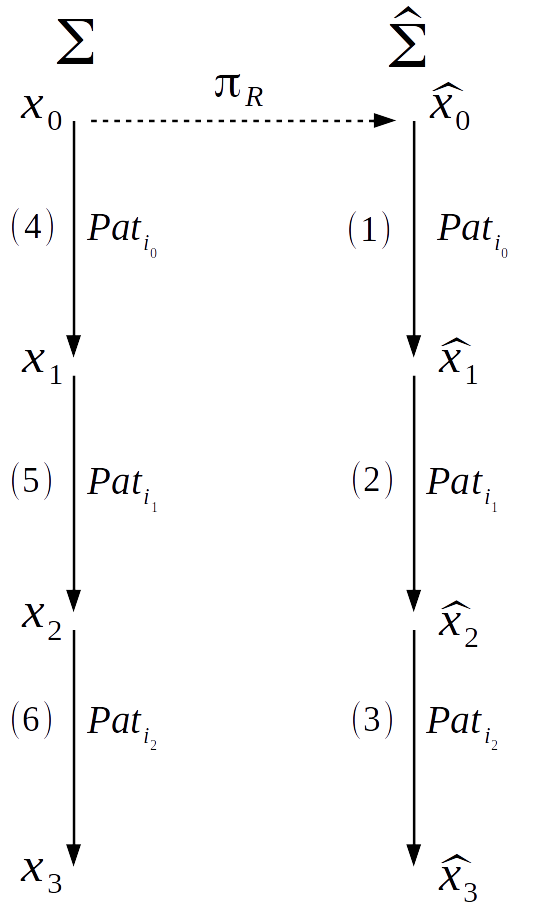
\includegraphics[width=39mm]{fig3.png}
  \caption{Diagram of the offline procedure for a simulation of length 3.}
 \label{fig:fig3}
\end{figure}

 This procedure thus allows, for any system $\Sigma$ of the form (\ref{eq:LTI}), 
 and given an interest set $R_x$ and an objective set~$R_y$, to send the output 
 of the full-order system in the set $R_y + \varepsilon_y^\infty$. More precisely,
 if $\hat \Sigma$ is the projection by balanced truncation of $\Sigma$, let $\hat \Delta$
 be a decomposition for ($\hat R_x$,$R_y$,$k)$ w.r.t. $\hat \Sigma$.
 Then, for all $x_0\in R_x$, the induced control $u_{\hat{\Delta}}$ applied to the full-order
 system $\Sigma$ in $x_0$ is such that for all $j>0$, the 
 output of the full-order system $y(t)$ returns to~$R_y + \varepsilon_y^\infty$ after
 at most $k$ $\tau$-steps.


Here, $R_y + \varepsilon_y^\infty$ denotes the set containing $R_y$ with a margin of $\varepsilon_y^\infty$.
If $R_y$ is an interval product of the form $\lbrack a_1,b_1 \rbrack \times \dots
\times \lbrack a_m,b_m \rbrack$, then $R_y + \varepsilon_y^\infty$ is defined by 
$\lbrack a_1 - \varepsilon_y^\infty,b_1 + \varepsilon_y^\infty \rbrack \times \dots \times
\lbrack a_m - \varepsilon_y^\infty,b_m +\varepsilon_y^\infty \rbrack$.

\vspace{1em}

{\bf Remark:}
 Here, we ensure that ${\bf y}(t,x_0,u)$ is in $R_y + \varepsilon_y^\infty$ at the end of every pattern, but an easy improvement is to ensure that ${\bf y}(t,x_0,u)$ stays in a safety set $S_y \supset R_y$ 
 at every step of time $k\tau$. Indeed, as explained in \cite{FKS-safety}, we can ensure that the unfolding of the output trajectory stays in a given safety set $S_y$.
 The unfolding of the output of a set is defined as follows:
 given a pattern $Pat$ of the form $(u_1\cdots u_m)$, and a set $X\subset\mathbb{R}^n$,
the {\em unfolding of the output of $X$ via~$Pat$}\index{unfolding}, 
denoted by $\mathit{Unf}_{Pat,C}(X)$, 
is the set $\bigcup_{i=0}^mX_i$ with:
\begin{itemize}
\item$X_0=\{ Cx \vert x \in X \} $,
\item $X_{i+1}=Post_{u_{i+1},C}(X_i)$, for all $0\leq i\leq m-1$.
\end{itemize}
The unfolding thus corresponds to the set of all the 
intermediate outputs produced when applying pattern $Pat$ to 
the states of $X$.
In order to guarantee that ${\bf y}(t,x_0,u)$ stays in $S_y$, we just have to make sure that ${\bf y_r}(t,\pi_Rx_0,u)$ stays in the reduced safety set $S_y - \varepsilon_y^\infty$.
We thus have to add, in the line $6$ of Algorithm~\ref{alg:findPat_part5}, the condition: ``and $\mathit{Unf}_{Pat,C}(W) \subset S_y -\varepsilon_y^\infty$''.






 \subsection{Semi-Online Procedure}
 

Up to this point, the procedure of control synthesis consists in computing a complete
sequence of patterns on the reduced order model $\hat \Sigma$ for a given initial 
state $x_0$, and applying the pattern sequence to the full-order model $\Sigma$. 
The entire control law is thus computed offline. While the decomposition
is always performed offline, one can however use the decomposition~$\hat \Delta$ online
as follows: let $x_0$ be the initial state in $R_x$ and $\hat x_0 = \pi_R x_0$  (step (1) of
Figure \ref{fig:fig4}) its projection
belonging to $\hat R_x$,~$\hat x_0$ belongs to $\hat V_{i_0}$ for some $i_0 \in I$; we can thus 
apply the associated pattern $Pat_{i_0}$ to the full-order system $\Sigma$, which yields
a state $x_1 = {\bf x}(\vert Pat_{i_0} \vert \tau,x_0,Pat_{i_0})$ (step (2) of Figure~\ref{fig:fig4}), the corresponding
output is sent to $y_1 = {\bf y}(\vert Pat_{i_0} \vert \tau,x_0,Pat_{i_0}) \in R_y + \varepsilon_y^{\vert Pat_{i_0} \vert}$; 
in order to continue to step (3), we have to guarantee that 
$\pi_R {\bf x}(\vert Pat_{i} \vert \tau,x,Pat_{i}))$ belongs to  $\hat R_x$ for all $x \in R_x$ and for all $i \in I$.
As explained below, this is possible using the computation of an upper bound to the
error 
 $\Vert \pi_R {\bf x}(\vert Pat_{i} \vert \tau,x,Pat_{i}) - {\hat {\bf x}}(\vert Pat_{i} \vert \tau,\pi_R x,Pat_{i}) \Vert $
and 
a reinforcement of the procedure for taking into account this error.


Let $\varepsilon_x^{\vert Pat \vert}$ be the upper bound to
 \[ \Vert \pi_R {\bf x}(\vert Pat \vert \tau,x,Pat) - {\hat {\bf x}}(\vert Pat \vert \tau,\pi_R x,Pat) \Vert, \]
as defined in equation (\ref{eq:boundx}).
We modify the Algorithms~\ref{alg:decompo_part5} and~\ref{alg:findPat_part5}, which
become ``Bisection$\_$\-Dyn'' and 
``Find$\_$Patt\-ern$\_$\-Dyn'' (Algorithms~\ref{alg:decompo2_part5} and~\ref{alg:findPat2_part5}),
they are computed with an additional input $\varepsilon_x = (\varepsilon_x^1,\dots,
\varepsilon_x^k)$, $k$ being the
maximal length of the patterns. With such an additional input, we perform
an {\em $\varepsilon$-decomposition}.
Given a system $\Sigma$, two sets $R_x$  and $R_y$ respectively subsets of ${\mathbb{R}^n}$
and  ${\mathbb{R}^m}$, a positive integer $k$, and a vector of errors $\varepsilon_x = (\varepsilon_x^1,\dots,
 \varepsilon_x^k)$,
application of the $\varepsilon$-decomposition
returns a set $\Delta$
of the form $\{V_i,Pat_i\}_{i \in I}$, where~$I$ is a finite set of indexes, every $V_i$ is a subset of $R_x$, and every $Pat_i$ is a $k$-pattern such that:
\begin{itemize} 
\item[(a')] $\bigcup_{i \in I}V_i = R_x$, 
\item[(b')] for all $i \in I$: $Post_{Pat_i}(V_i) \subseteq R_x - \varepsilon_x^{\vert Pat_i \vert}$,
\item[(c')] for all $i \in I$: $Post_{Pat_i,C}(V_i) \subseteq R_y$.
\end{itemize}


Note that condition (b') is a strengthening of condition (b) in subsection \ref{sec:ssda}.
Accordingly, line 6 of Algorithm \ref{alg:findPat_part5} becomes in Algorithm~\ref{alg:findPat2_part5}:
{
\[
\textbf{6} \quad \textbf{if} ~{Post_{Pat}(W) \subseteq R_x - \varepsilon_x^i ~and ~Post_{Pat,C}(W) \subseteq R_y } ~\textbf{then}
\]
}
The new algorithms enable to guarantee that the projection of the full-order system state~$\pi_R x$
always stays in $\hat R_x$, we can thus perform the online control as follows:

Since $Post_{Pat_{i_0}}(\hat V_{i_0}) \subseteq \hat R_x - \varepsilon_x^{\vert Pat_{i_0} \vert}$
and $\pi_R x_0 \in \hat V_{i_0}$,
we have $Post_{Pat_{i_0}}(\pi_R x_0) \in \hat R_x - \varepsilon_x^{\vert Pat_{i_0} \vert}$;
thus  $\pi_R x_1 = \pi_R {\bf x}(\vert Pat_{i_0} \vert \tau,x_0,Pat_{i_0})$ belongs to $\hat R_x$, because $\varepsilon_x^{\vert Pat_{i_0} \vert}$
is a bound of the maximal distance between ${\bf \hat x}(\vert Pat_{i_0} \vert \tau,\pi_R x_0,Pat_{i_0})$
and $\pi_R {\bf x}(\vert Pat_{i_0} \vert \tau,x_0,Pat_{i_0})$; \linebreak
 since $\pi_R x_1$ belongs to $\hat R_x$, it belongs to $V_{i_1}$ for some $i_1 \in I$; we can thus compute the input pattern $Pat_{i_1}$,
and therefore, we can reapply the procedure and compute an input pattern sequence $Pat_{i_0}$,$Pat_{i_1}$,$\dots$
As for the output, the yielded points $y_1 = {\bf y} (\vert Pat_{i_0} \vert \tau, x_0, Pat_{i_0})$, 
$y_2 = {\bf y} (\vert Pat_{i_1} \vert \tau, x_1, Pat_{i_1})$, $\dots$ belong respectively 
to the sets $R_y + \varepsilon_y^{\vert Pat_{i_0} \vert}$,$R_y + \varepsilon_y^{\vert Pat_{i_1} \vert}$,$\dots$



\begin{figure}[ht]
\centering
 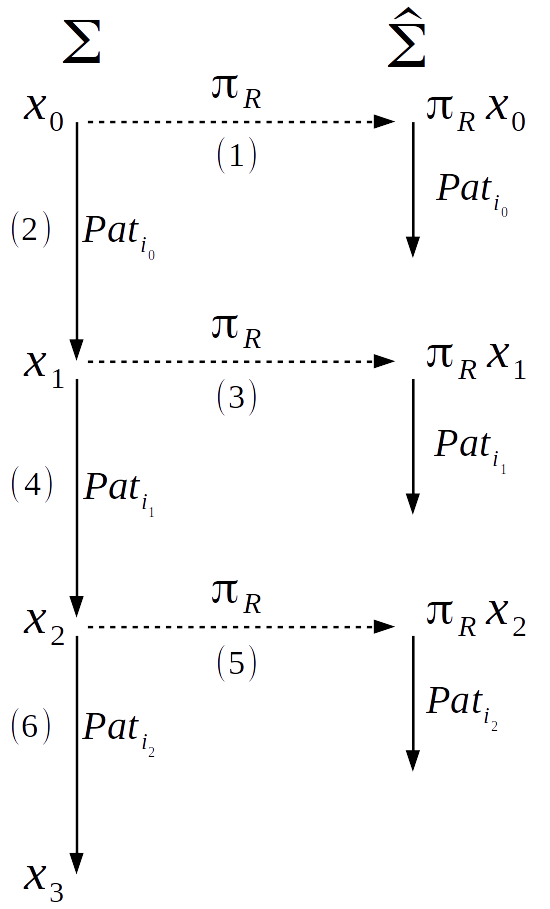
\includegraphics[width=39mm]{fig4.png}
 \caption{Diagram of the online procedure for a simulation of length 3.}
 \label{fig:fig4}
\end{figure}

 The main advantage of such an online control is that the estimated errors $\varepsilon_y^{\vert Pat_{i_0} \vert}$,$\varepsilon_y^{\vert Pat_{i_1} \vert}$,$\dots$
are dynamically computed, and are smaller than the static bound $\varepsilon_y^\infty$ used
in the offline control. The price to be paid is the strengthening of
condition (b'). In the best case, i.e. if the errors are low and the system is very contractive,
this can result in the same decomposition and computation time as in the offline procedure.
But if the system is not contractive enough or if the errors are too large, this can 
lead to a more complicated decomposition, and thus higher computation times,
and in the worst case, no successful decomposition at all. 
 
 
 \begin{algorithm}[ht]
 \centering
 \begin{algorithmic}
 \STATE{{\bf Input:} A box $W$, a box $R_x$, a box $R_y$, a length $K$ of pattern, a vector of errors $\varepsilon_x$, a degree $D$ of bisection}
  \STATE{{\bf Output:} $\langle\{(V_i,Pat_i)\}_{i},True\rangle$ with $\bigcup_i V_i=W$,
$\bigcup_i Post_{Pat_i}(V_i)\subseteq R_x$ and $\bigcup_i Post_{Pat_i,C}(V_i)\subseteq R_y$,  %and $\bigcup_i Unf_{Pat_i}(V_i)\subseteq S$
or $\langle\_ ,False\rangle$}
  \STATE{$(Pat,b) := $Find$\_$Pattern$\_$Dyn$(W,R_x,R_y,K,\varepsilon_x)$}\\
  \IF{$b=True$}{
    \STATE{{\bf return} $\langle\{(W,Pat)\},True\rangle$}
  }
  \ELSE
      \IF{$D=0$}{
	  \RETURN{$\langle\_ ,False\rangle$}
       }
       \ELSE \STATE{Divide equally $W$ into $(W_1,\dots, W_{2^{n}})$ }\ \ \ \\
	    \FOR{$i=1\dots2^{n}$}\STATE{
	      $(\Delta_i,b_i)$ := Decomposition$\_$Dyn($W_i$,$R_x$,$R_y$,$K$,$\varepsilon_x$,$D - 1$)\\
	    }
	    \ENDFOR
 	      \RETURN{$(\bigcup_{i=1\dots 2^{n}} \Delta_i,\bigwedge_{i=1\dots 2^{n}} b_i)$}
 	\ENDIF    
\ENDIF
 \end{algorithmic}
\caption{{\small Decomposition\_Dyn($W,R_x,R_y,D,K,\varepsilon_x$)}}  
\label{alg:decompo2_part5}  
\end{algorithm}

\begin{algorithm}[ht]
\centering
\begin{algorithmic}
 \STATE{{\bf Input:} A box $W$, a box $R_x$, a box $R_y$, a length $K$ of pattern, a vector of errors $\varepsilon_x$}
 \STATE{{\bf Output:} $\langle Pat,True\rangle$ with ,$Post_{Pat}(W)\subseteq R_x$,$Post_{Pat,C}(W)\subseteq R_y$ and $Unf_{Pat}(W)\subseteq S$, or $\langle\_, False\rangle$ when 
no pattern maps $W$ into $R_x$ and $CW$ into $R_y$}
   \FOR{$i=1\dots K$}\STATE{$\Pi :=$ set of patterns of length $i$}\\
    \WHILE{$\Pi$ is non empty} \STATE{Select $Pat$ in $\Pi$\\ $\Pi:= \Pi\setminus  \{Pat\}$\\} \IF{$Post_{Pat}(W) \subseteq R_x - \varepsilon_x^i$ and $Post_{Pat,C}(W) \subseteq R_y $}
    {\RETURN{$\langle Pat,True\rangle$}}\ENDIF
    \ENDWHILE
    \ENDFOR
   \RETURN{$\langle\_ ,False\rangle$}
\end{algorithmic}
   \caption{\small Find\_Pattern\_Dyn($W,R_x,R_y,K,\varepsilon_x$)}
\label{alg:findPat2_part5}
\end{algorithm}

 
 
 \section{Numerical Results}
 \label{sec:examples}
  \subsection{Thermal Problem on a Metal Plate}
  \label{sec:thermal}

  \begin{figure}[ht]
\centering
 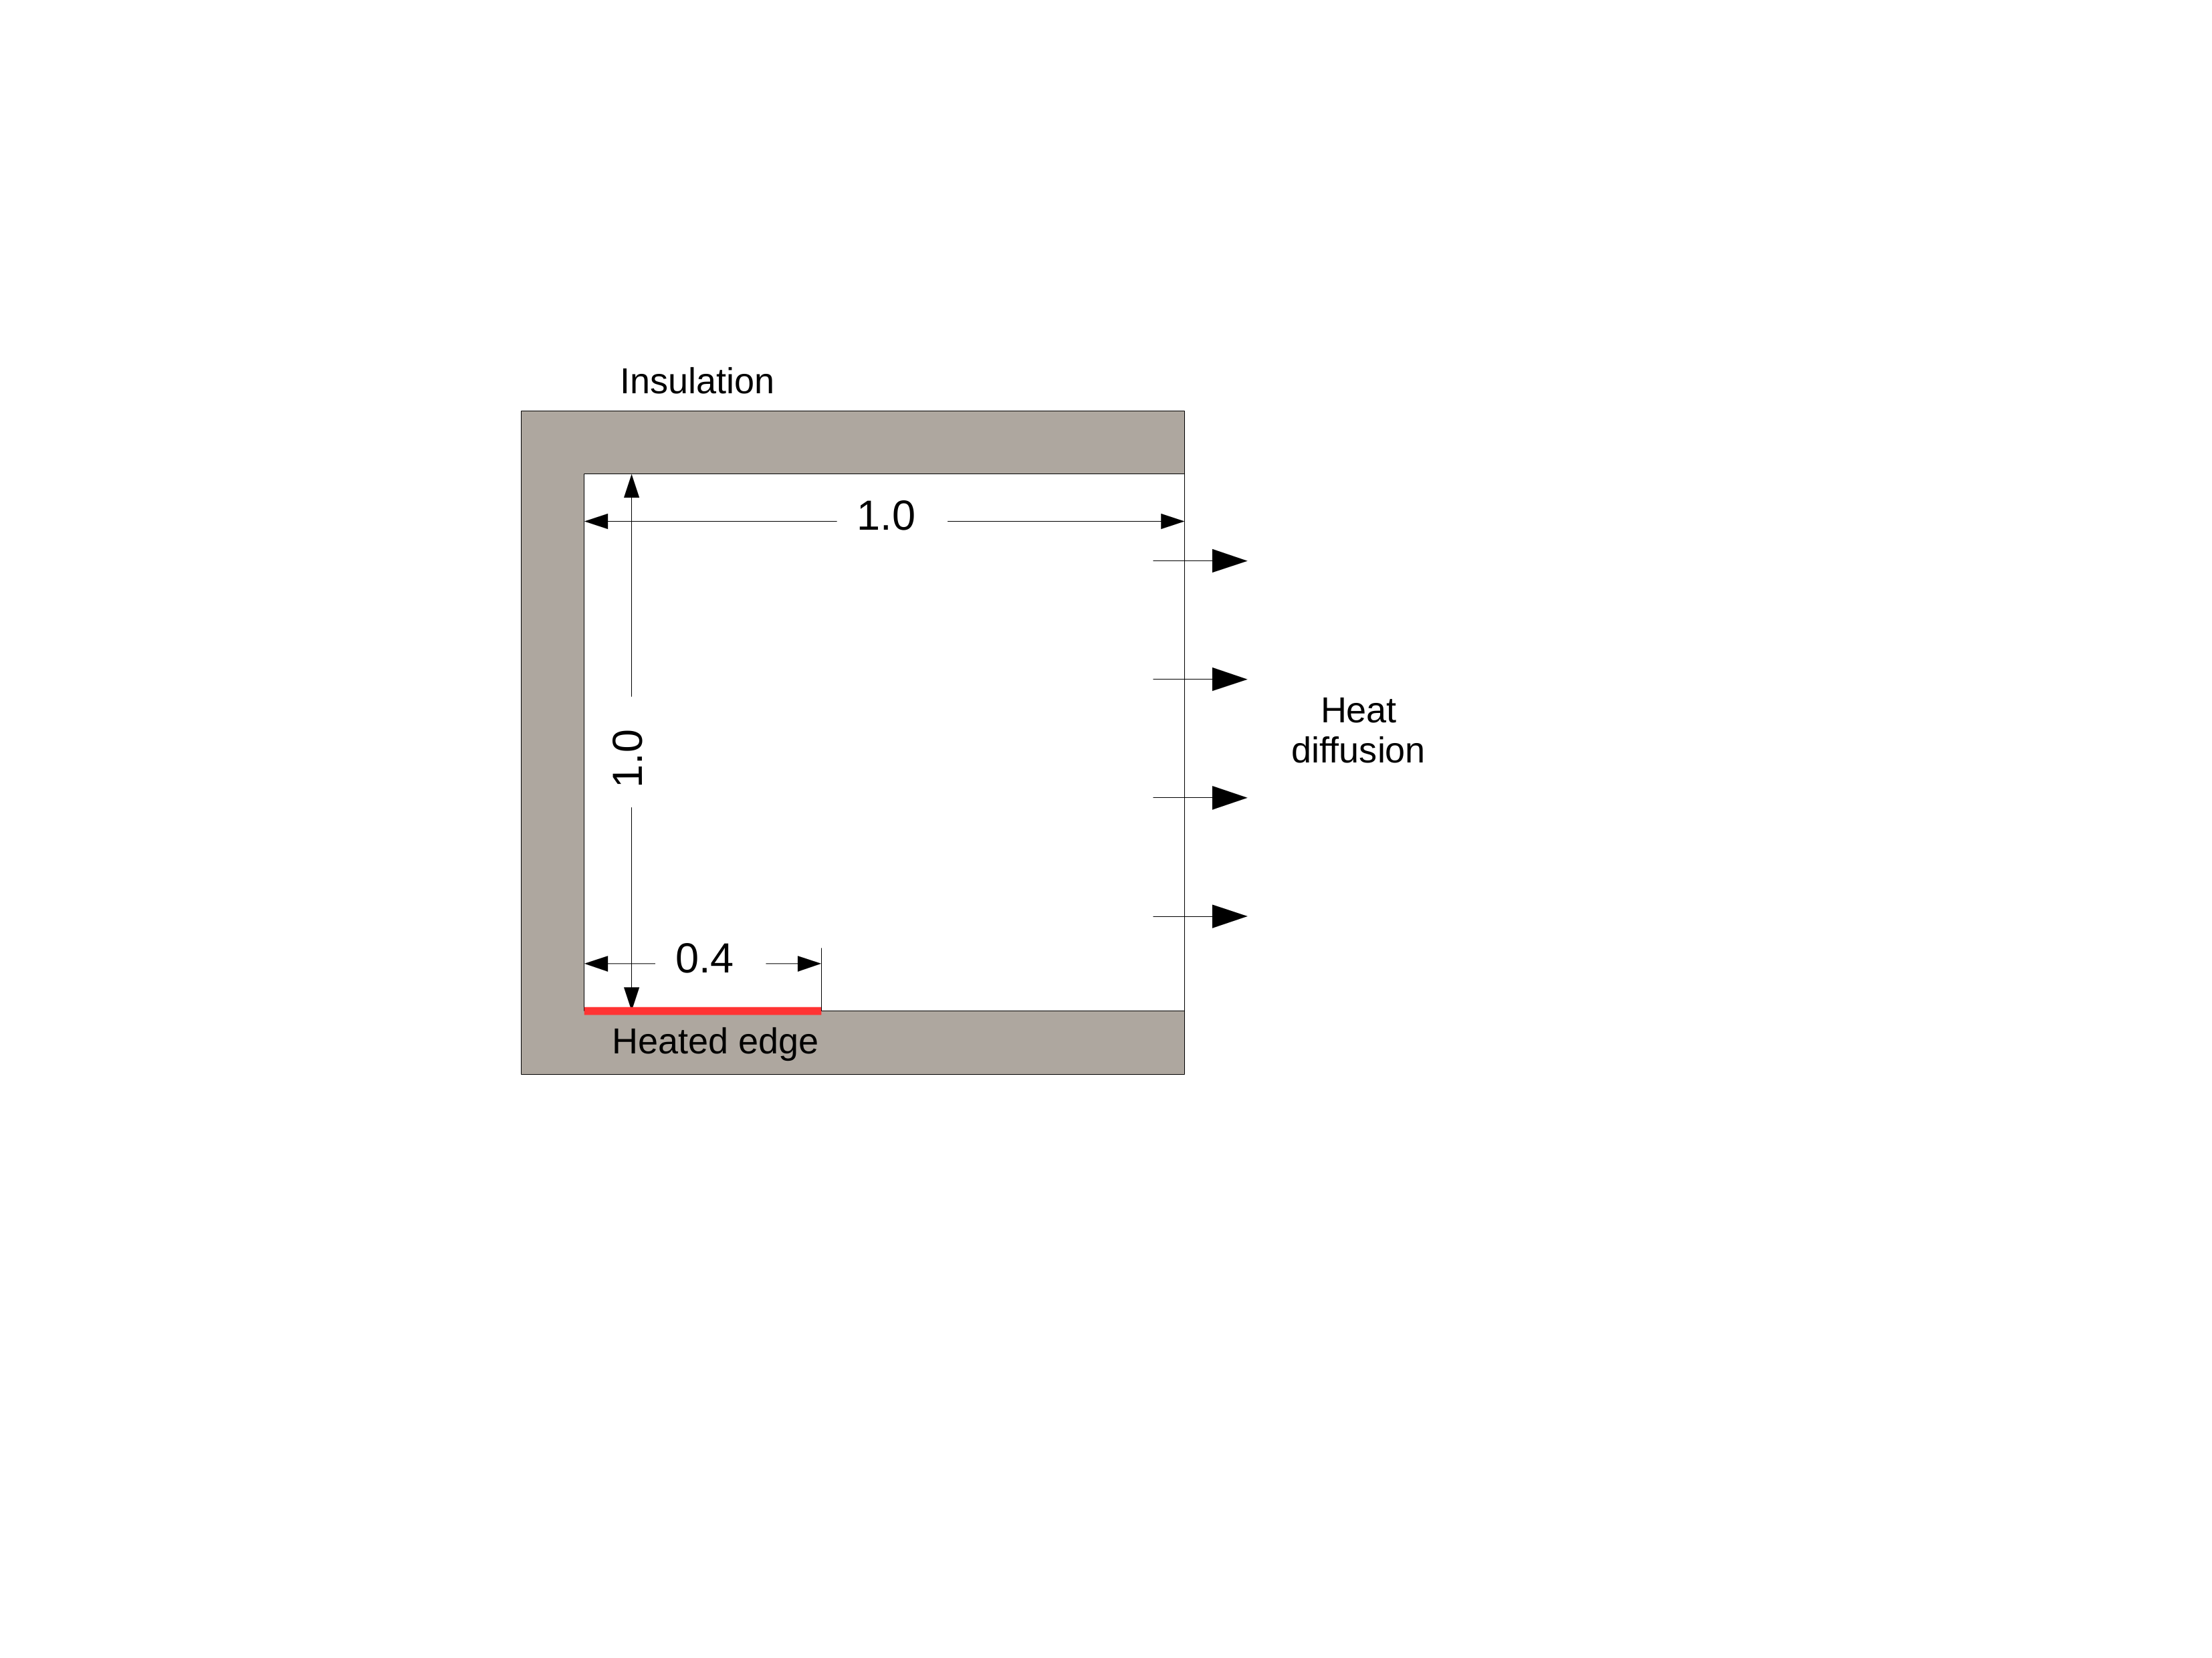
\includegraphics[trim = 2cm 7cm 5cm 4cm, clip, width=84mm]{fig5.png}
\caption{Geometry of the square plate.}
\label{fig:fig5}
\end{figure}
  
We consider here the problem of controlling the central node temperature of a square metal plate,
discretized by finite elements; this example
is taken from \cite{han_krogh_06}. The square plate is subject to the heat equation: 
$\dfrac{\partial T}{\partial t}(x,t) - \alpha \Delta T(x,t) = 0$.
After discretization, the system is written under its state-space representation (\ref{eq:LTI}). 
The plate is insulated along three edges, while the right edge is open. The left half
of the bottom edge is connected to a heat source. The exterior temperature
is set to $0^\circ$C, the temperature of the heat source is either $0^\circ$C (mode~$0$) or $1^\circ$C (mode $1$).
The heat transfers with the exterior and the heat source are modeled by a 
convective transfer. 
The full-order system state corresponds to the nodal temperatures. The output
is the temperature of the central node. The system is reduced from
$n=897$ to $n_r=2$ (Figure \ref{fig:fig7}) and $n_r=3$ (Figure \ref{fig:fig8}). The interest set is $R_x = \lbrack 0 , 0.15 \rbrack^{897}$ and the objective
set $R_y = \lbrack 0.06 , 0.09 \rbrack$. The sampling time is set to $\tau = 8$~s. 
The geometry of the system is given in Figure \ref{fig:fig5}. The decomposition obtained
with the offline procedure is given in Figure \ref{fig:fig6}. 

The decompositions and simulations have been performed with MINIMATOR 
(an Octave code available at https://bitbucket.org/alecoent/minimator$\_$red)
on a 2.80 GHz Intel Core i7-4810MQ CPU with 8 GB of memory.
The decompositions were obtained in $5$ seconds for the case $n_r=2$ and in $2$ minutes
for the case $n_r=3$.

\begin{figure}[ht]
 \centering
 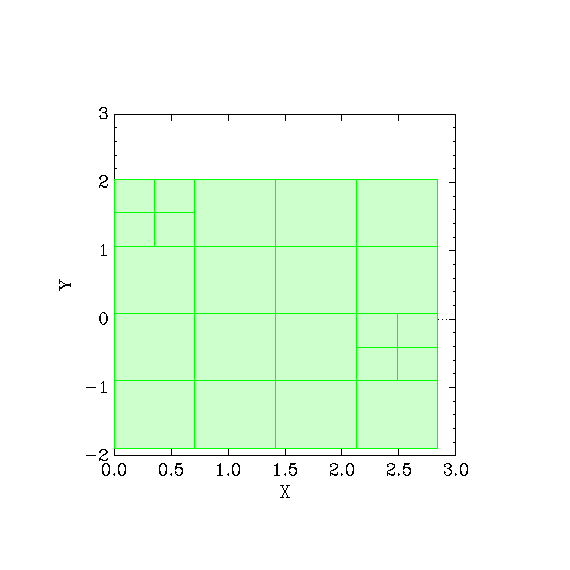
\includegraphics[trim= 50 70 100 100,clip=true,width=39mm]{fig6.png}
\caption{Decomposition of $\hat R_x = \pi_R R_x$ in the plane 
$(\hat x_1, \hat x_2)$ (for $n_r=2$) with the offline procedure.}
\label{fig:fig6}
\end{figure}


Simulations of the offline and online methods are given in Figures \ref{fig:fig7}
and \ref{fig:fig8}. 
We notice in Figure \ref{fig:fig7} that the trajectory $y$ (resp. $y_r$) exceeds the objective set 
$R_y$ (resp. $R_y + \varepsilon_y^{\vert Pat_i \vert}$) during the application of the second pattern,
yet the markers corresponding to the end of input patterns do belong to objective sets.
Comparing the cases $n_r=2$ and $n_r=3$, we finally observe that a less reduced model 
causes lower error bounds, and thus a more precise control, at the expense of a higher computation time.





\begin{figure}[ht!]
\centering
 \begin{tabular}{cc} 
 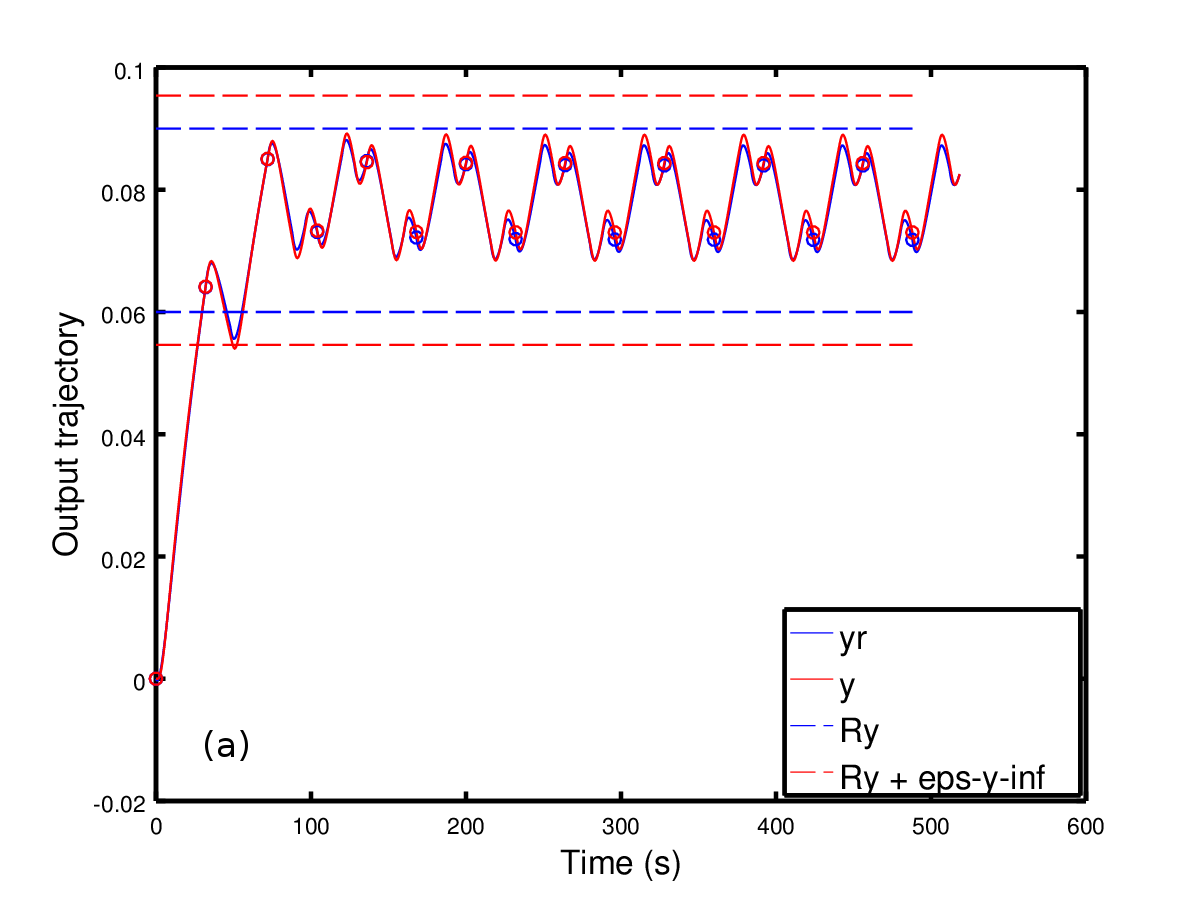
\includegraphics[width=0.48\textwidth]{fig7a.png}
 & 
 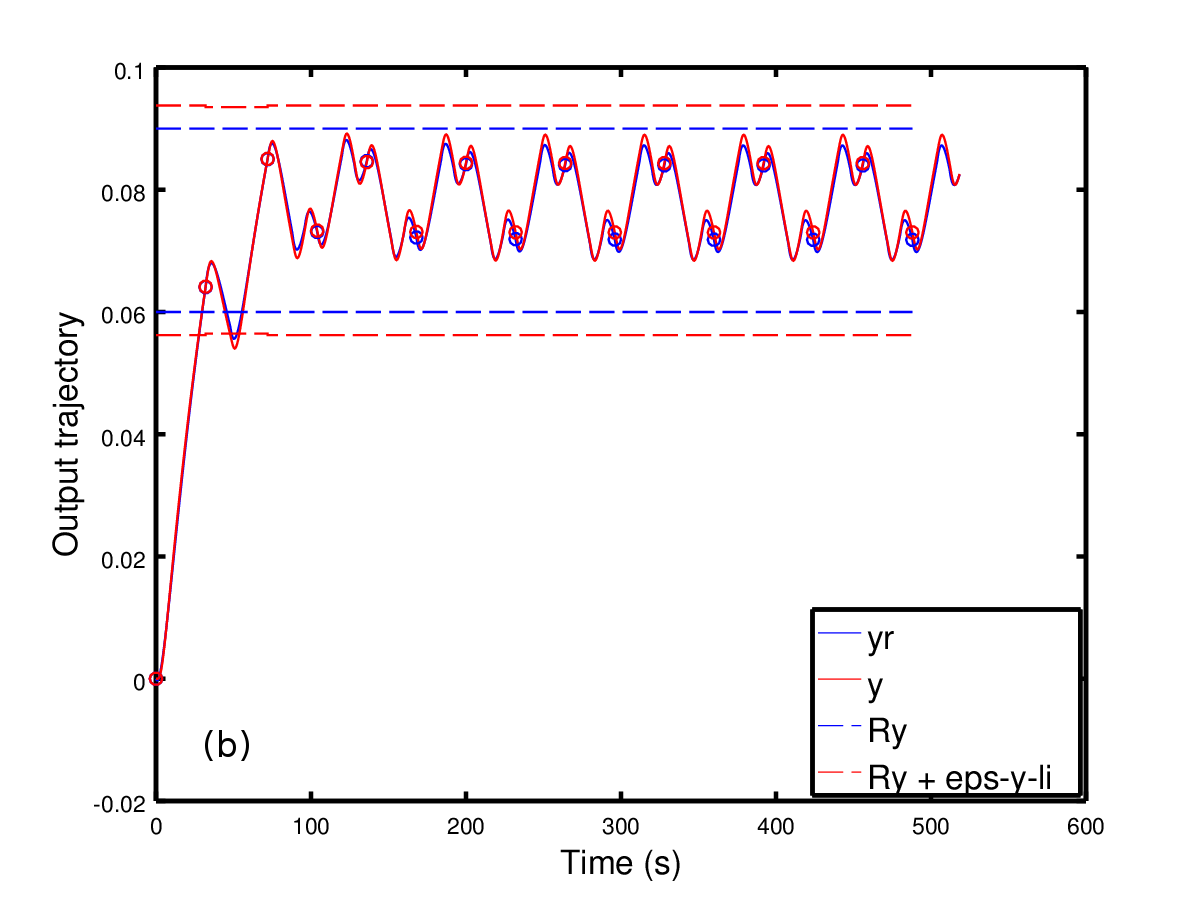
\includegraphics[width=0.48\textwidth]{fig7b.png}
 \end{tabular}
 \caption{For $n_r=2$, simulation of $y(t) = Cx(t)$ and $y_r(t) = \hat C \hat x(t)$ 
 from the initial condition~$x_0=(0)^{897}$. (a): guaranteed offline control; (b): guaranteed online control.}
 \label{fig:fig7}
\end{figure}
  
\begin{figure}[ht!]
\centering
 \begin{tabular}{cc} 
 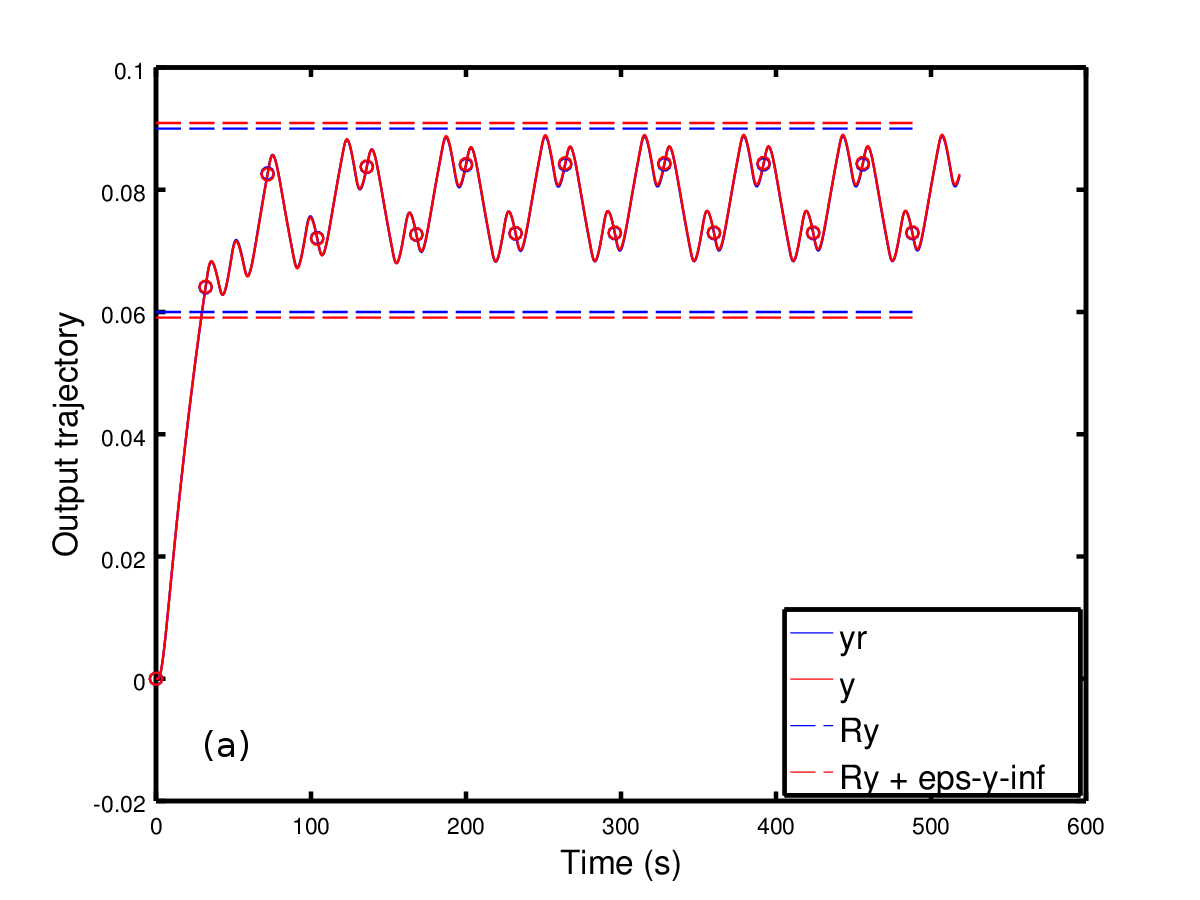
\includegraphics[width=0.48\textwidth]{fig8a.png}
 & 
 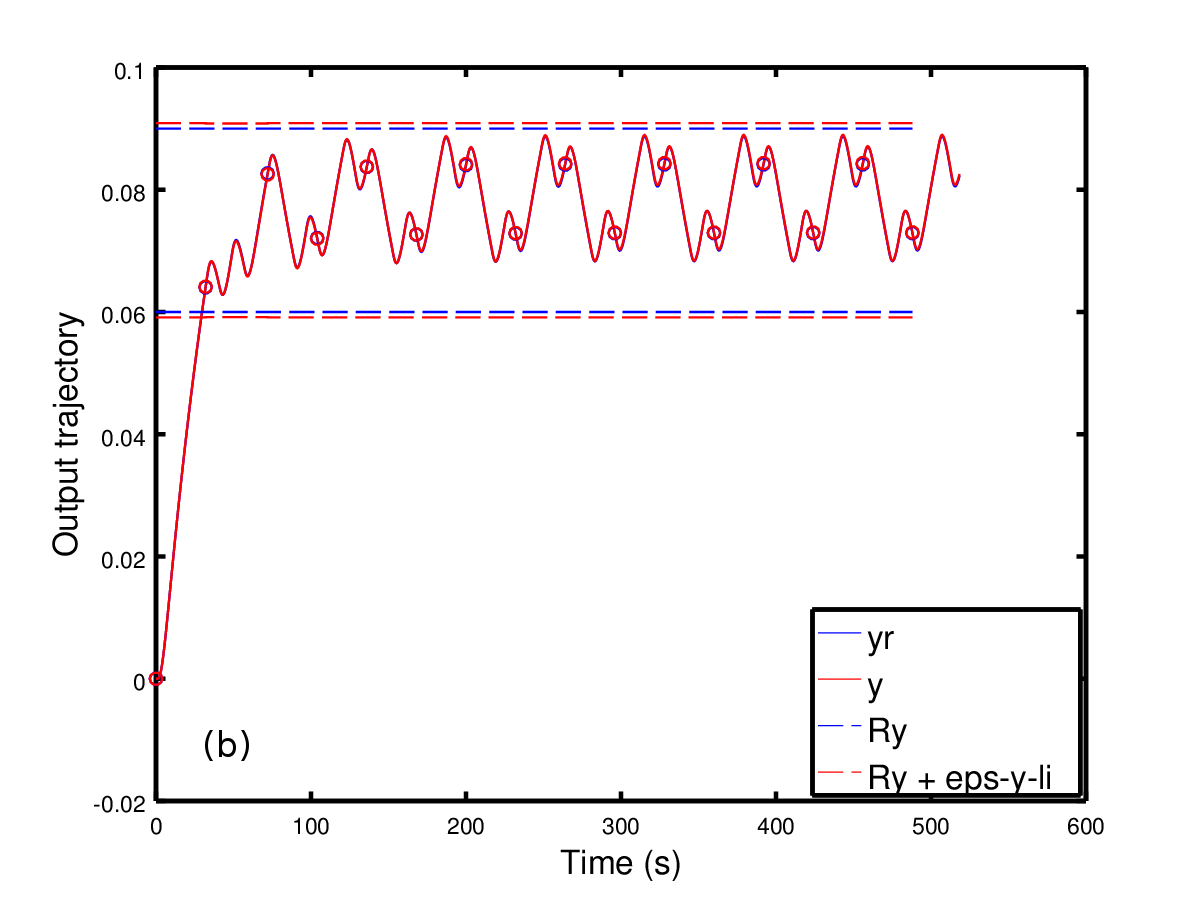
\includegraphics[width=0.48\textwidth]{fig8b.png}
 \end{tabular}
 \caption{For $n_r=3$, simulation of $y(t) = Cx(t)$ and $y_r(t) = \hat C \hat x(t)$ 
 from the initial condition~$x_0=(0)^{897}$. (a): guaranteed offline control; (b): guaranteed online control.}
 \label{fig:fig8}
\end{figure}  
  
  
  \subsection{Vibrating Beam}
  
    \begin{figure}
    \centering
  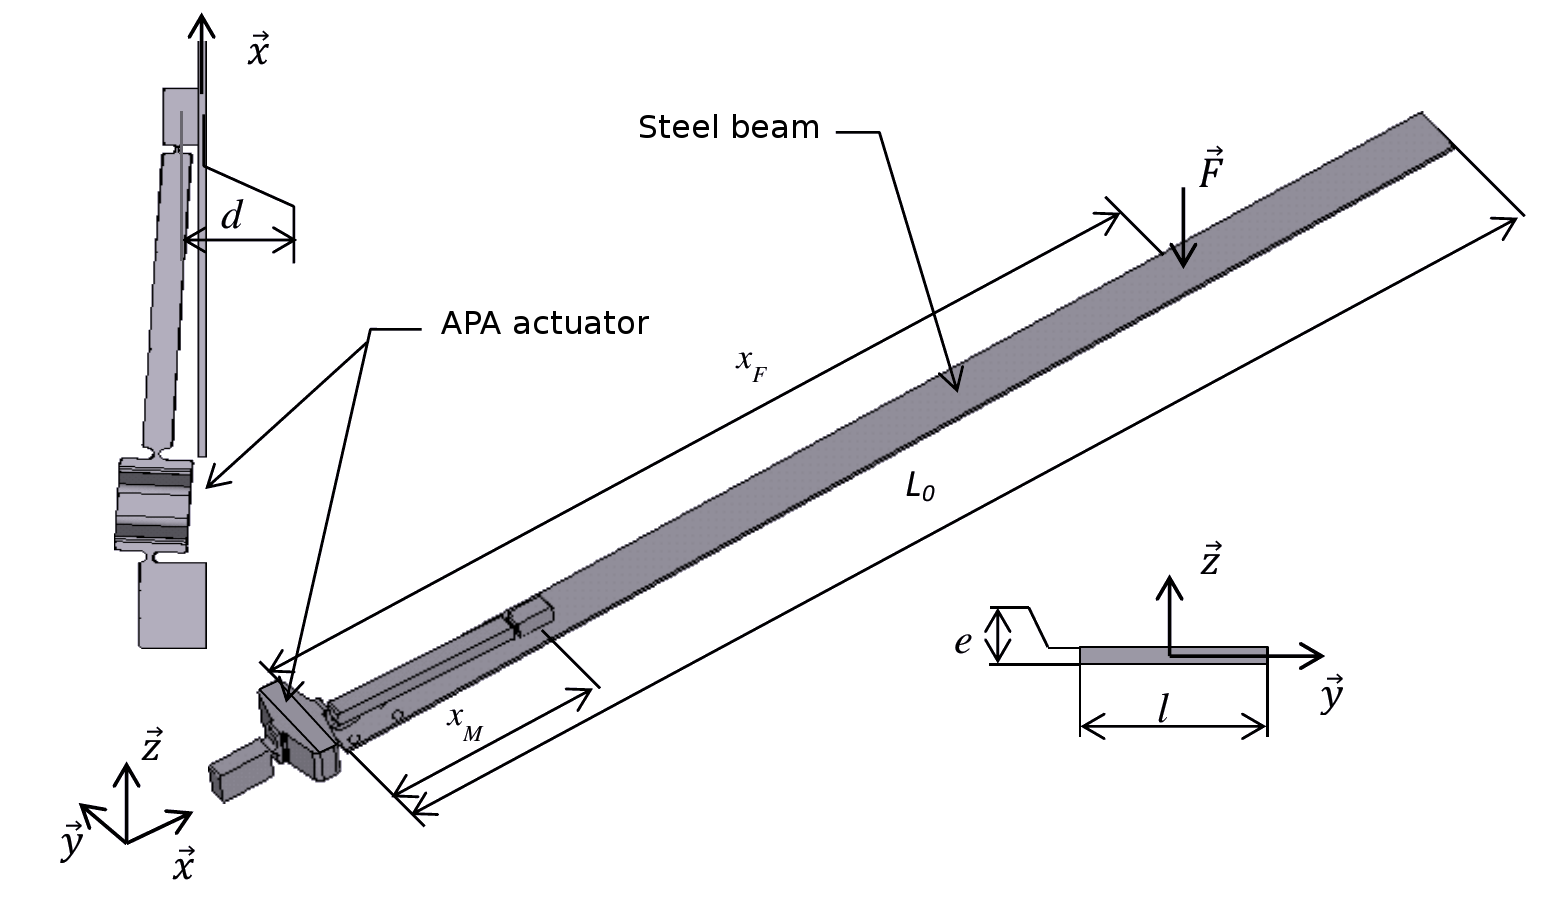
\includegraphics[width=0.6\textwidth]{fig9.png}
  \caption{Scheme of the vibrating beam.}
  \label{fig:fig9}
  \end{figure}
  In this case study, which comes from a practical work designed by Fabien Formosa \cite{formosa},
  we apply our method to vibration  control of a cantilever beam.
  The objective is to keep the tip displacement of the beam as close as possible to zero.
  To stabilize the beam, a piezoelectric patch applies a torque with the mechanism schemed in
  Figure \ref{fig:fig9} at a distance $x_M$ from the blocked side of the beam.
  The model retained is a finite element model with classical beam elements.
  The beam equation is the following:
  \begin{equation}
   m \ddot{w}(x,t) + EI \dfrac{\partial^4 w(x,t)}{\partial x^ 4} = \dfrac{\partial M_u}{\partial x}
   \delta(x - x_M)
  \end{equation}
  The torque $M_u$ is chosen with the control variable $u$. By applying the 
  right torque at the right time, we hope to stabilize the beam.
  In its finite element writing, the system is:
  \begin{equation}
   M \ddot{W} + K W = F_u
      \label{eq:EF_vib}
  \end{equation}
  Using a modal decomposition 
  \[\displaystyle W(x,t) = \sum_{i\leq {n_{modes}}} a_i(t) \varphi_i(x),\]
  we can write a reduced system of the form:
  \begin{equation}
   M_r \ddot{a}_i(t) + 2 \zeta_i \dot{a}_i(t) + K_r a_i(t) = F_{r,u}.
   \label{eq:modal}
  \end{equation}
  Note that a modal damping is added in this step, it permits to have a realistic behaviour
  of the beam since it is subject to loss of energy.
  By rearranging the terms
  of equation~\eqref{eq:modal} into
  a first order ODE, we can write the system under a state-space representation:
\begin{equation}
 \Sigma : \left\lbrace
\begin{array}{ll}
\dot x(t) & = A x(t)+B u(t), \\
 y(t) & =C x(t),
\end{array}
\right.
\label{eq:LTI2}
\end{equation}
 where the output $y$ is the tip displacement of the beam. Henceforth, the state variable contains
 the variables $a_i$ and $\dot a_i$. The dimension of the state-space is thus twice the number
 of retained modes. In this way, the system can be treated with the method developed here, applying a
 balanced truncation to the system (\ref{eq:LTI2}) and building a reduced-order control.
  
  Note that the intermediate model order reduction by modal decomposition cannot actually be avoided, because 
  the direct rearrangement of system \eqref{eq:EF_vib} into its state-space representation leads
  to a matrix $A$ possessing some positive eigenvalues (instead of only negative ones),
  and the calculation of balancing transformations is then much more complicated, or even impossible.
 
 The finite element model is composed of $60$ elements (thus $120$ degrees of
 freedom to take the rotation into account), we retain $20$ modes 
 for the modal decomposition, and the system is reduced to $n_r = 4$.
 Nine control modes are chosen to control the beam, including the mode
 corresponding to a null torque.
 Two simulations for different initial conditions and
 objective sets are given in Figure \ref{fig:fig10}.
 In the first one, several modes are initially excited, whereas only the first mode is 
 excited in the second one. 
 In both cases, the online procedure is applied, 
 and we manage to stabilize the tip displacement relatively fast.
 The output of the full-order system is stabilized in $R_y + \varepsilon_y^{\vert Pat_i \vert}$
 with $\varepsilon_y^{\vert Pat_i \vert} \backsimeq 0.2$. The errors $\varepsilon_y^{\vert Pat_i \vert}$
 can seem quite high compared to the tip displacement, this comes from the hyperbolic
 nature of the equations which rule this example. However, in a practical point of view, this 
 is clear that the reduced-order output fits well the behavior of the full-order system.
  
  
  \begin{figure}[ht]
  \centering
   \begin{tabular}{cc}
    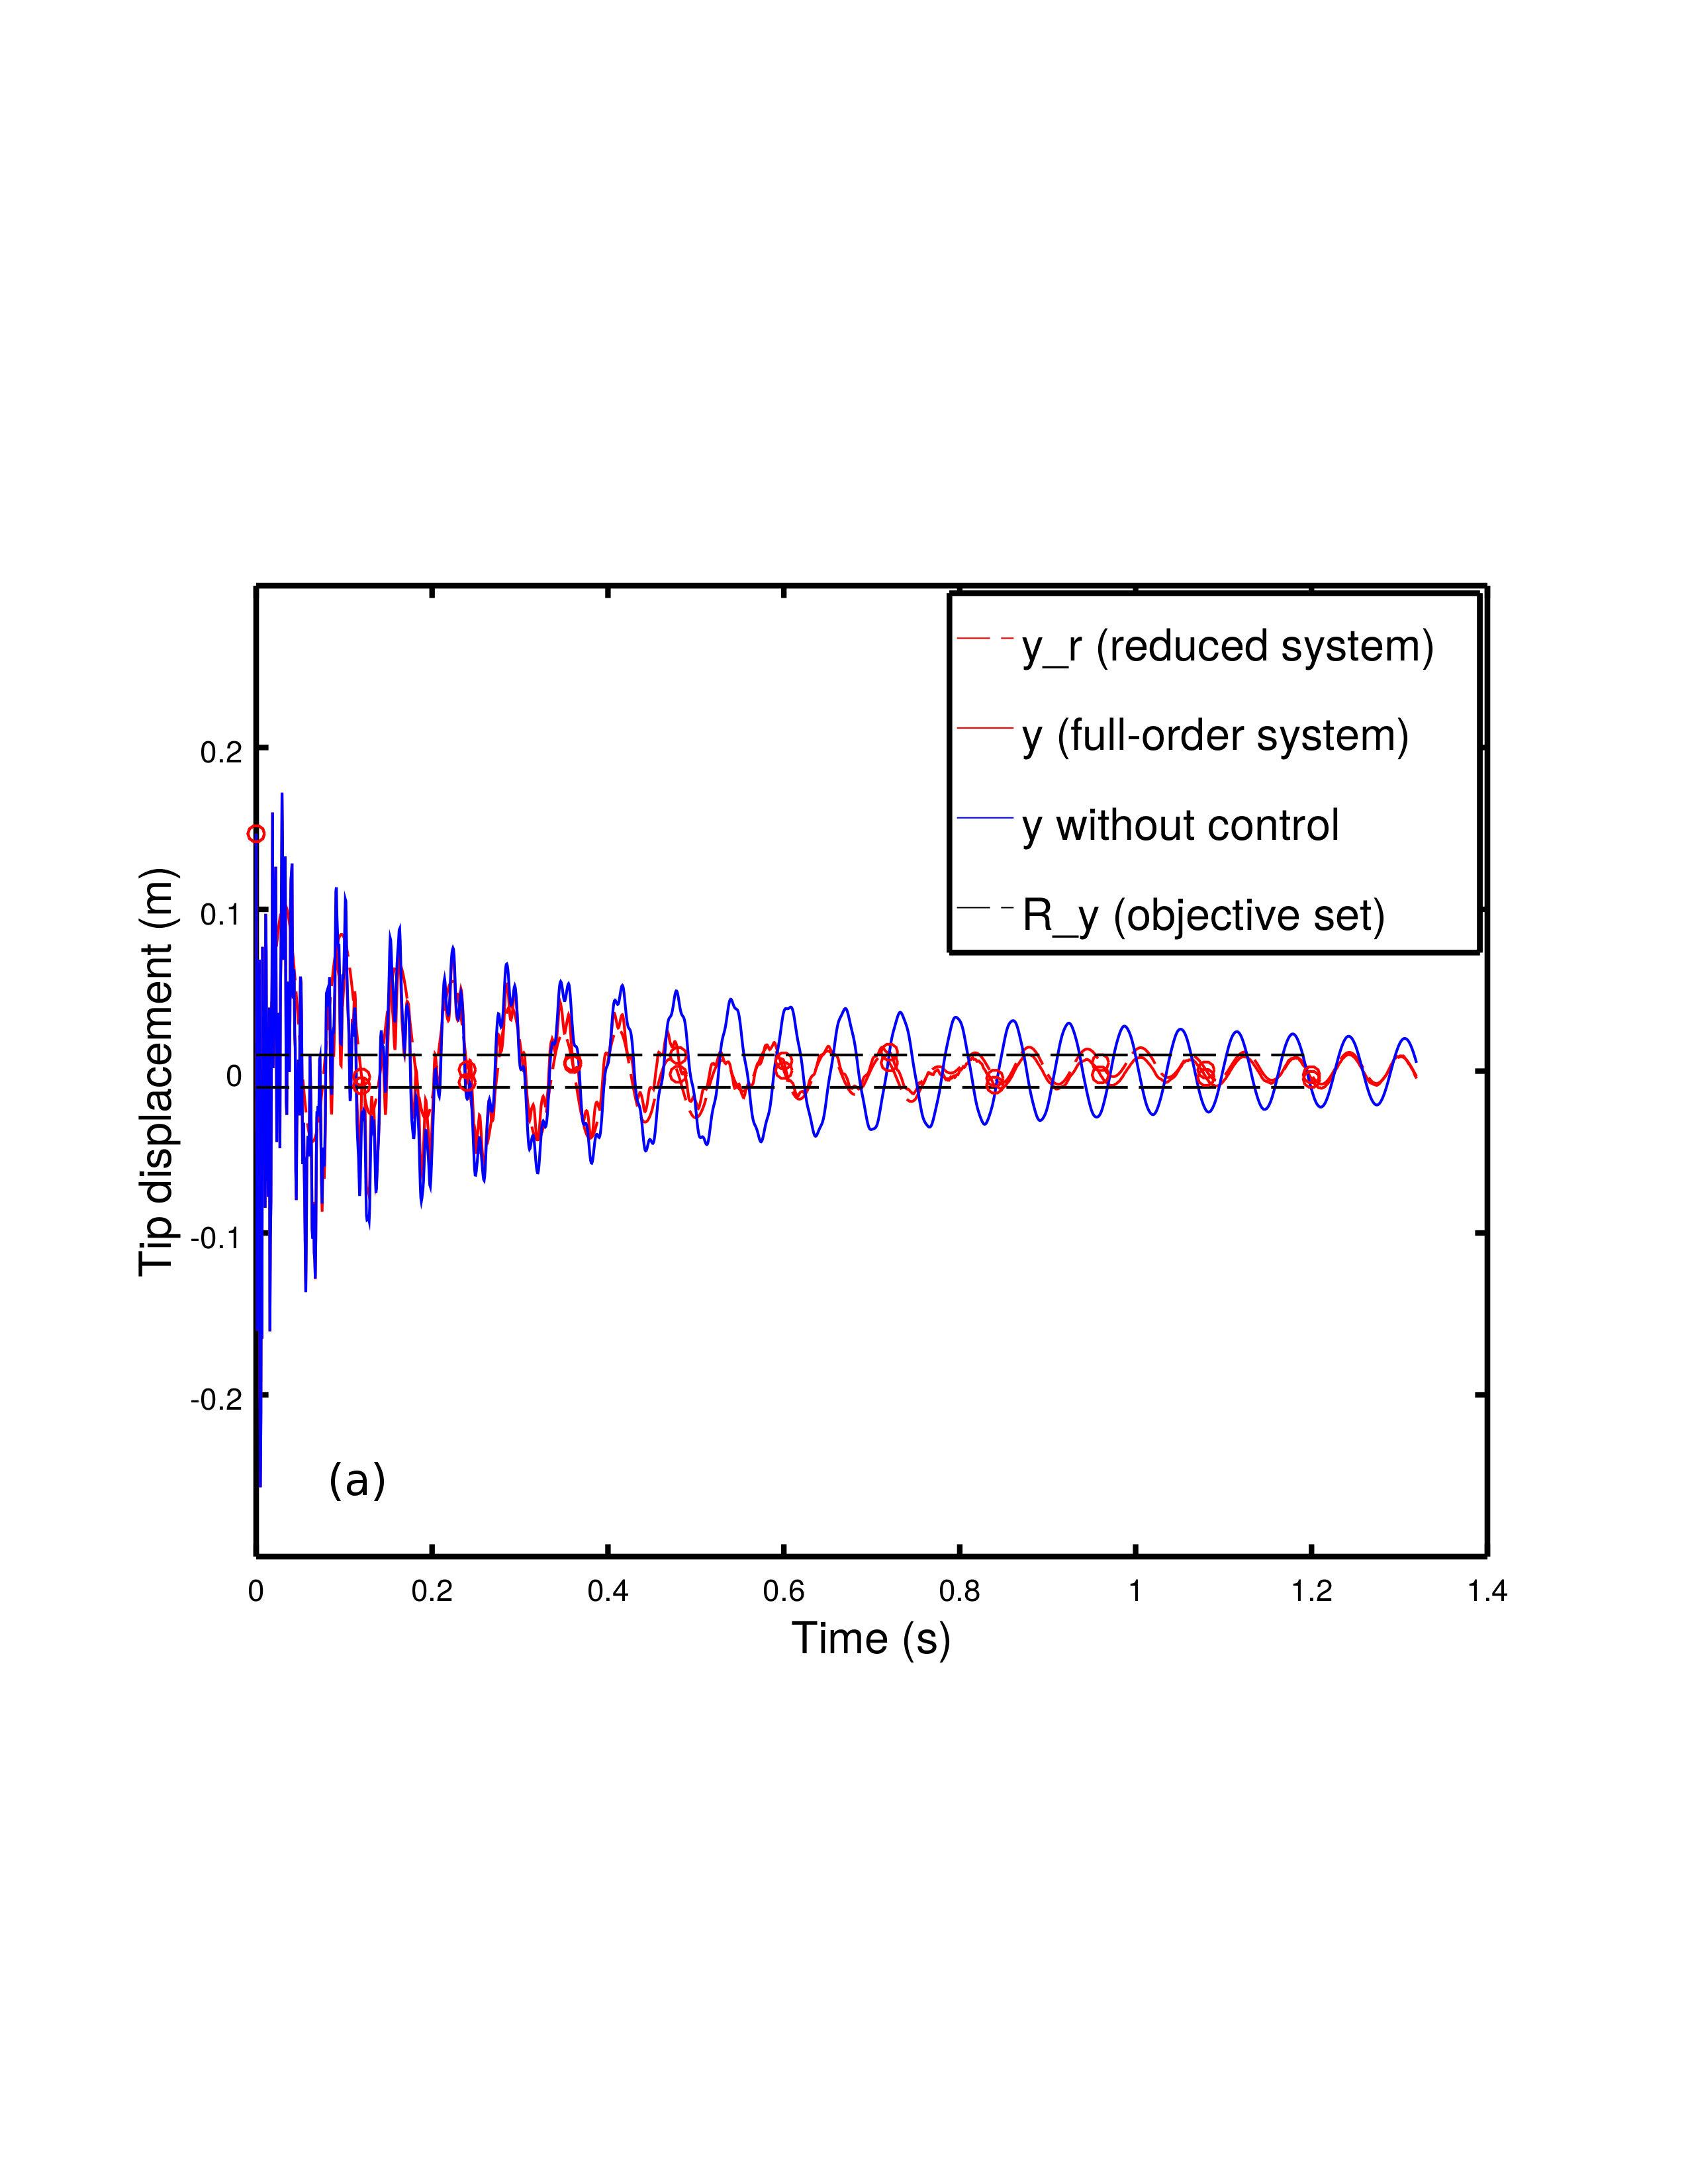
\includegraphics[trim = 0.8cm 6cm 0.8cm 6cm,clip,width=0.48\textwidth]{fig10a.png}
    & 
    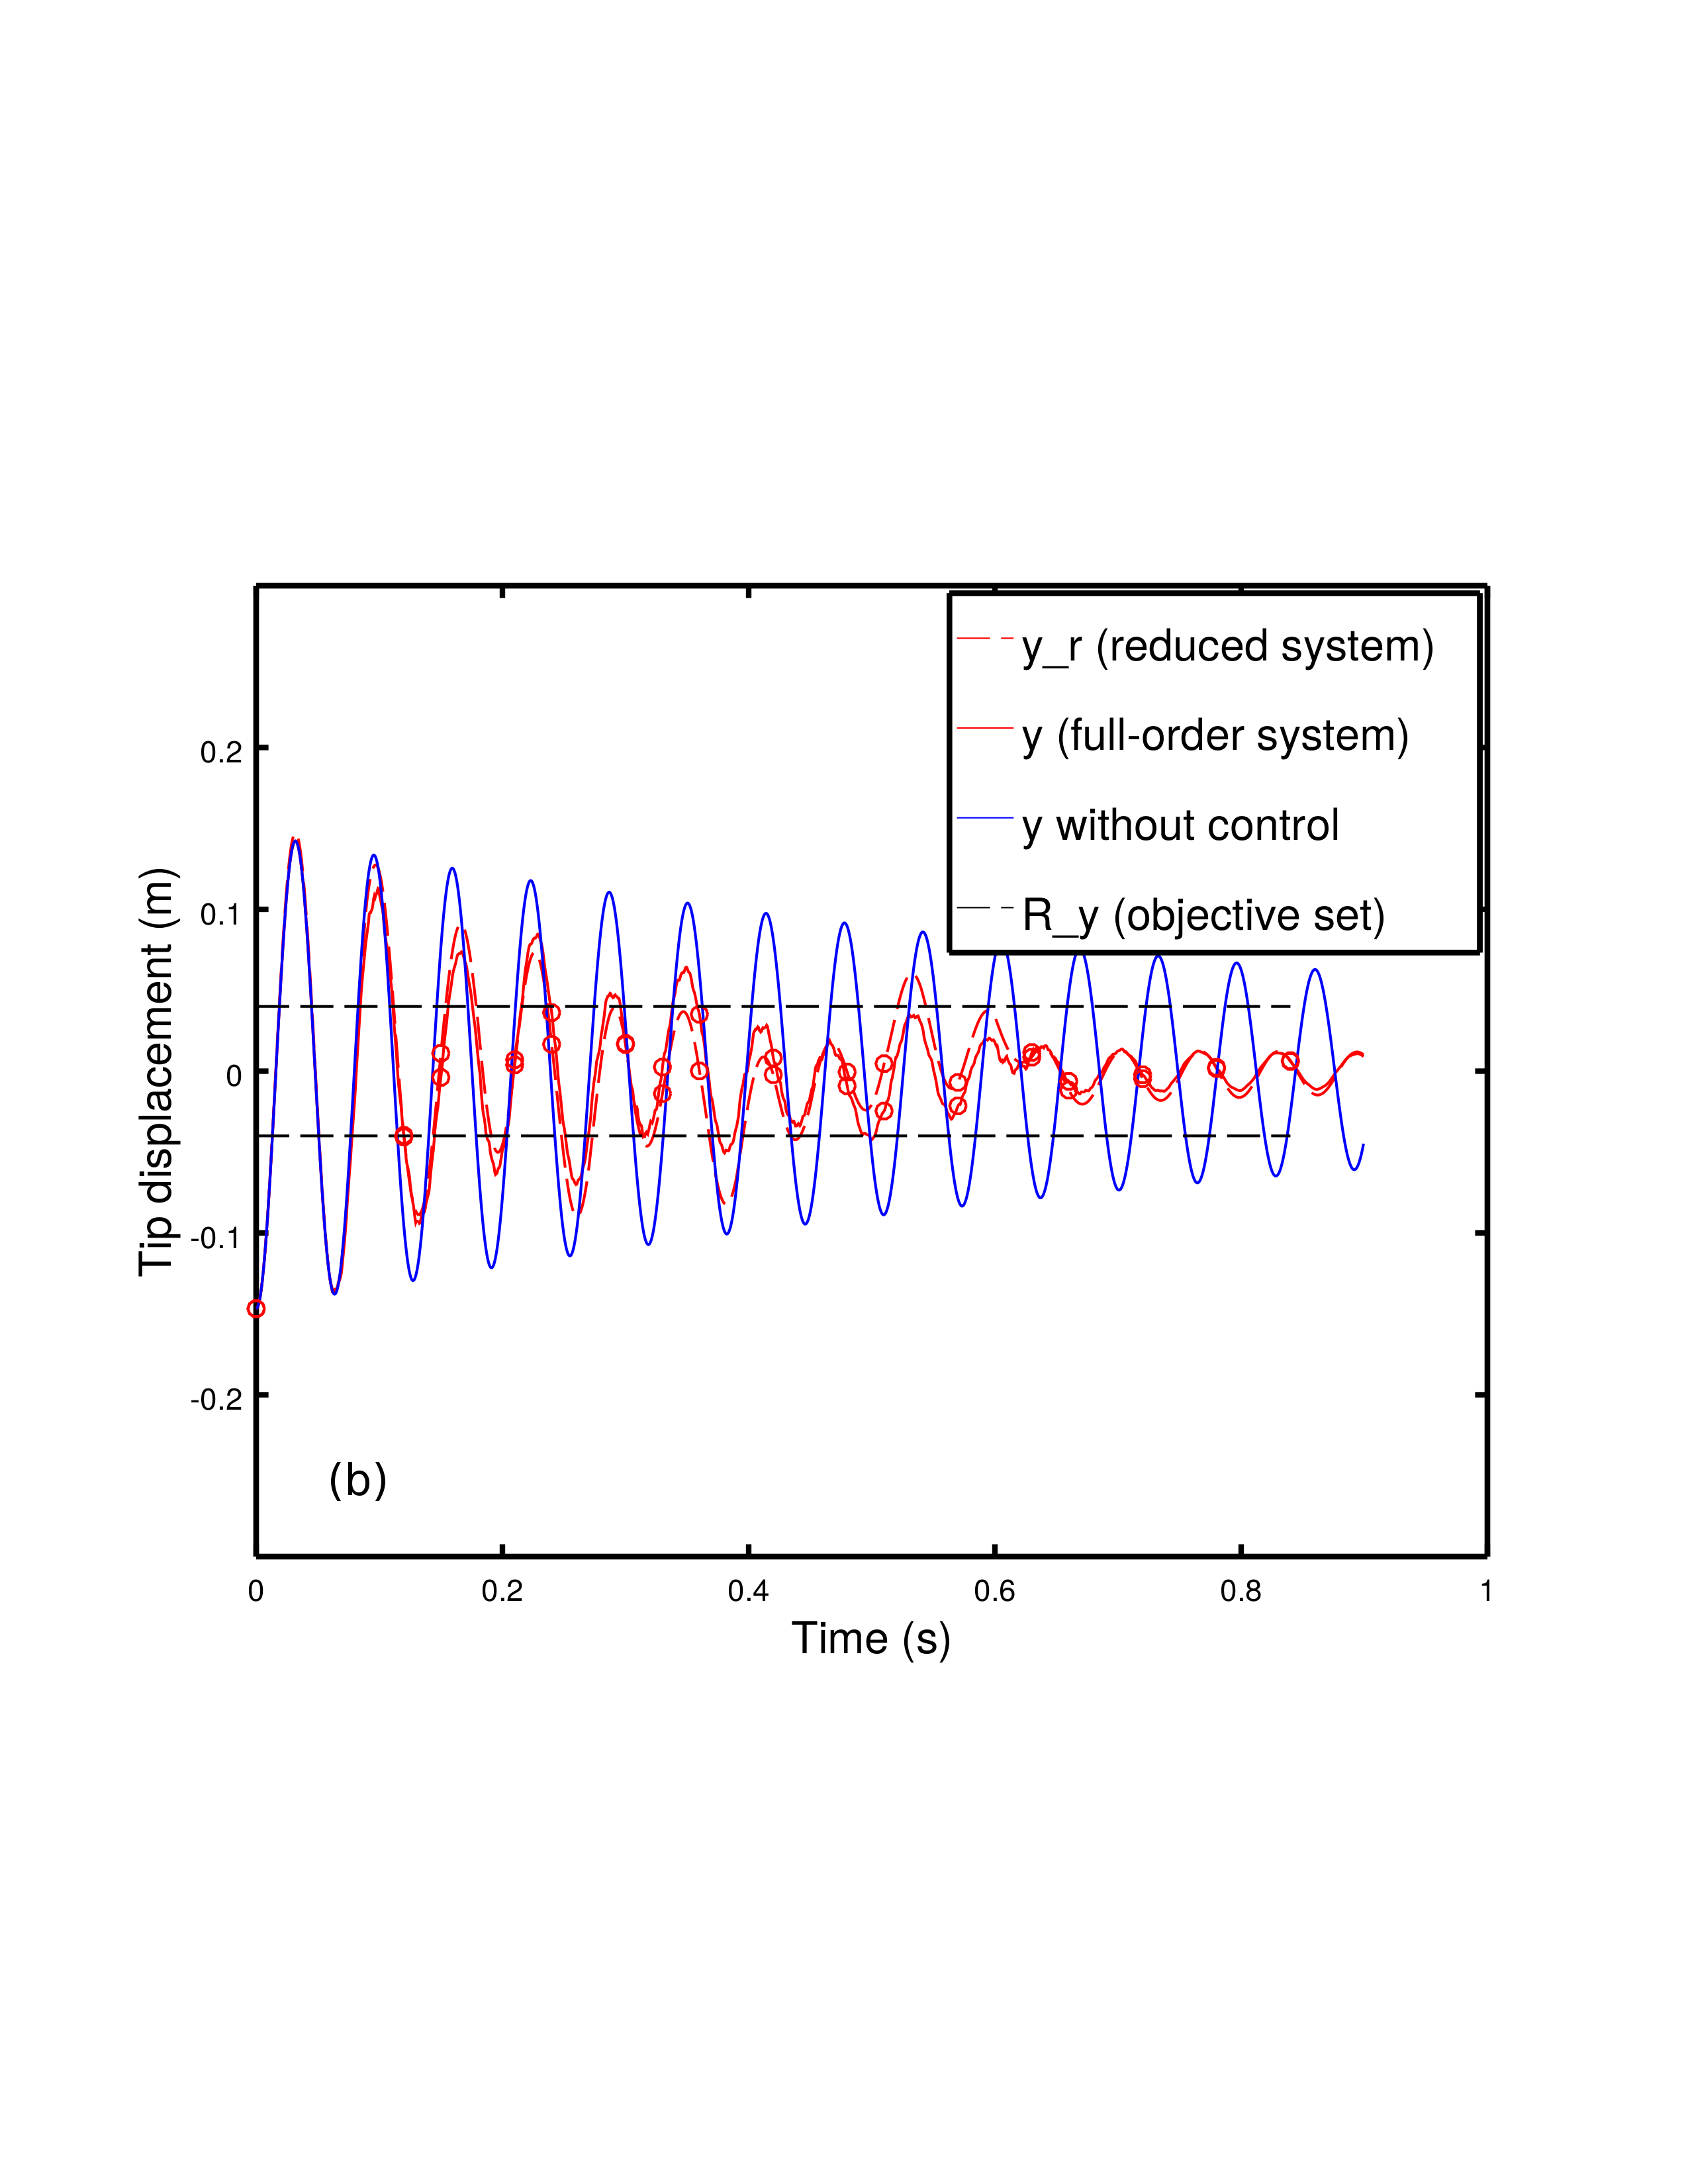
\includegraphics[trim = 0.8cm 6cm 0.8cm 6cm,clip,width=0.48\textwidth]{fig10b.png}
   \end{tabular}
  \caption{Simulations of vibration control of the cantilever beam for two different initial conditions and objective boxes. (a):~several modes excited; (b): first mode excited.}
  \label{fig:fig10}
  \end{figure}

  
  \subsection{Vibrating Aircraft Panel}
 
    \begin{figure}[ht]
    \centering
  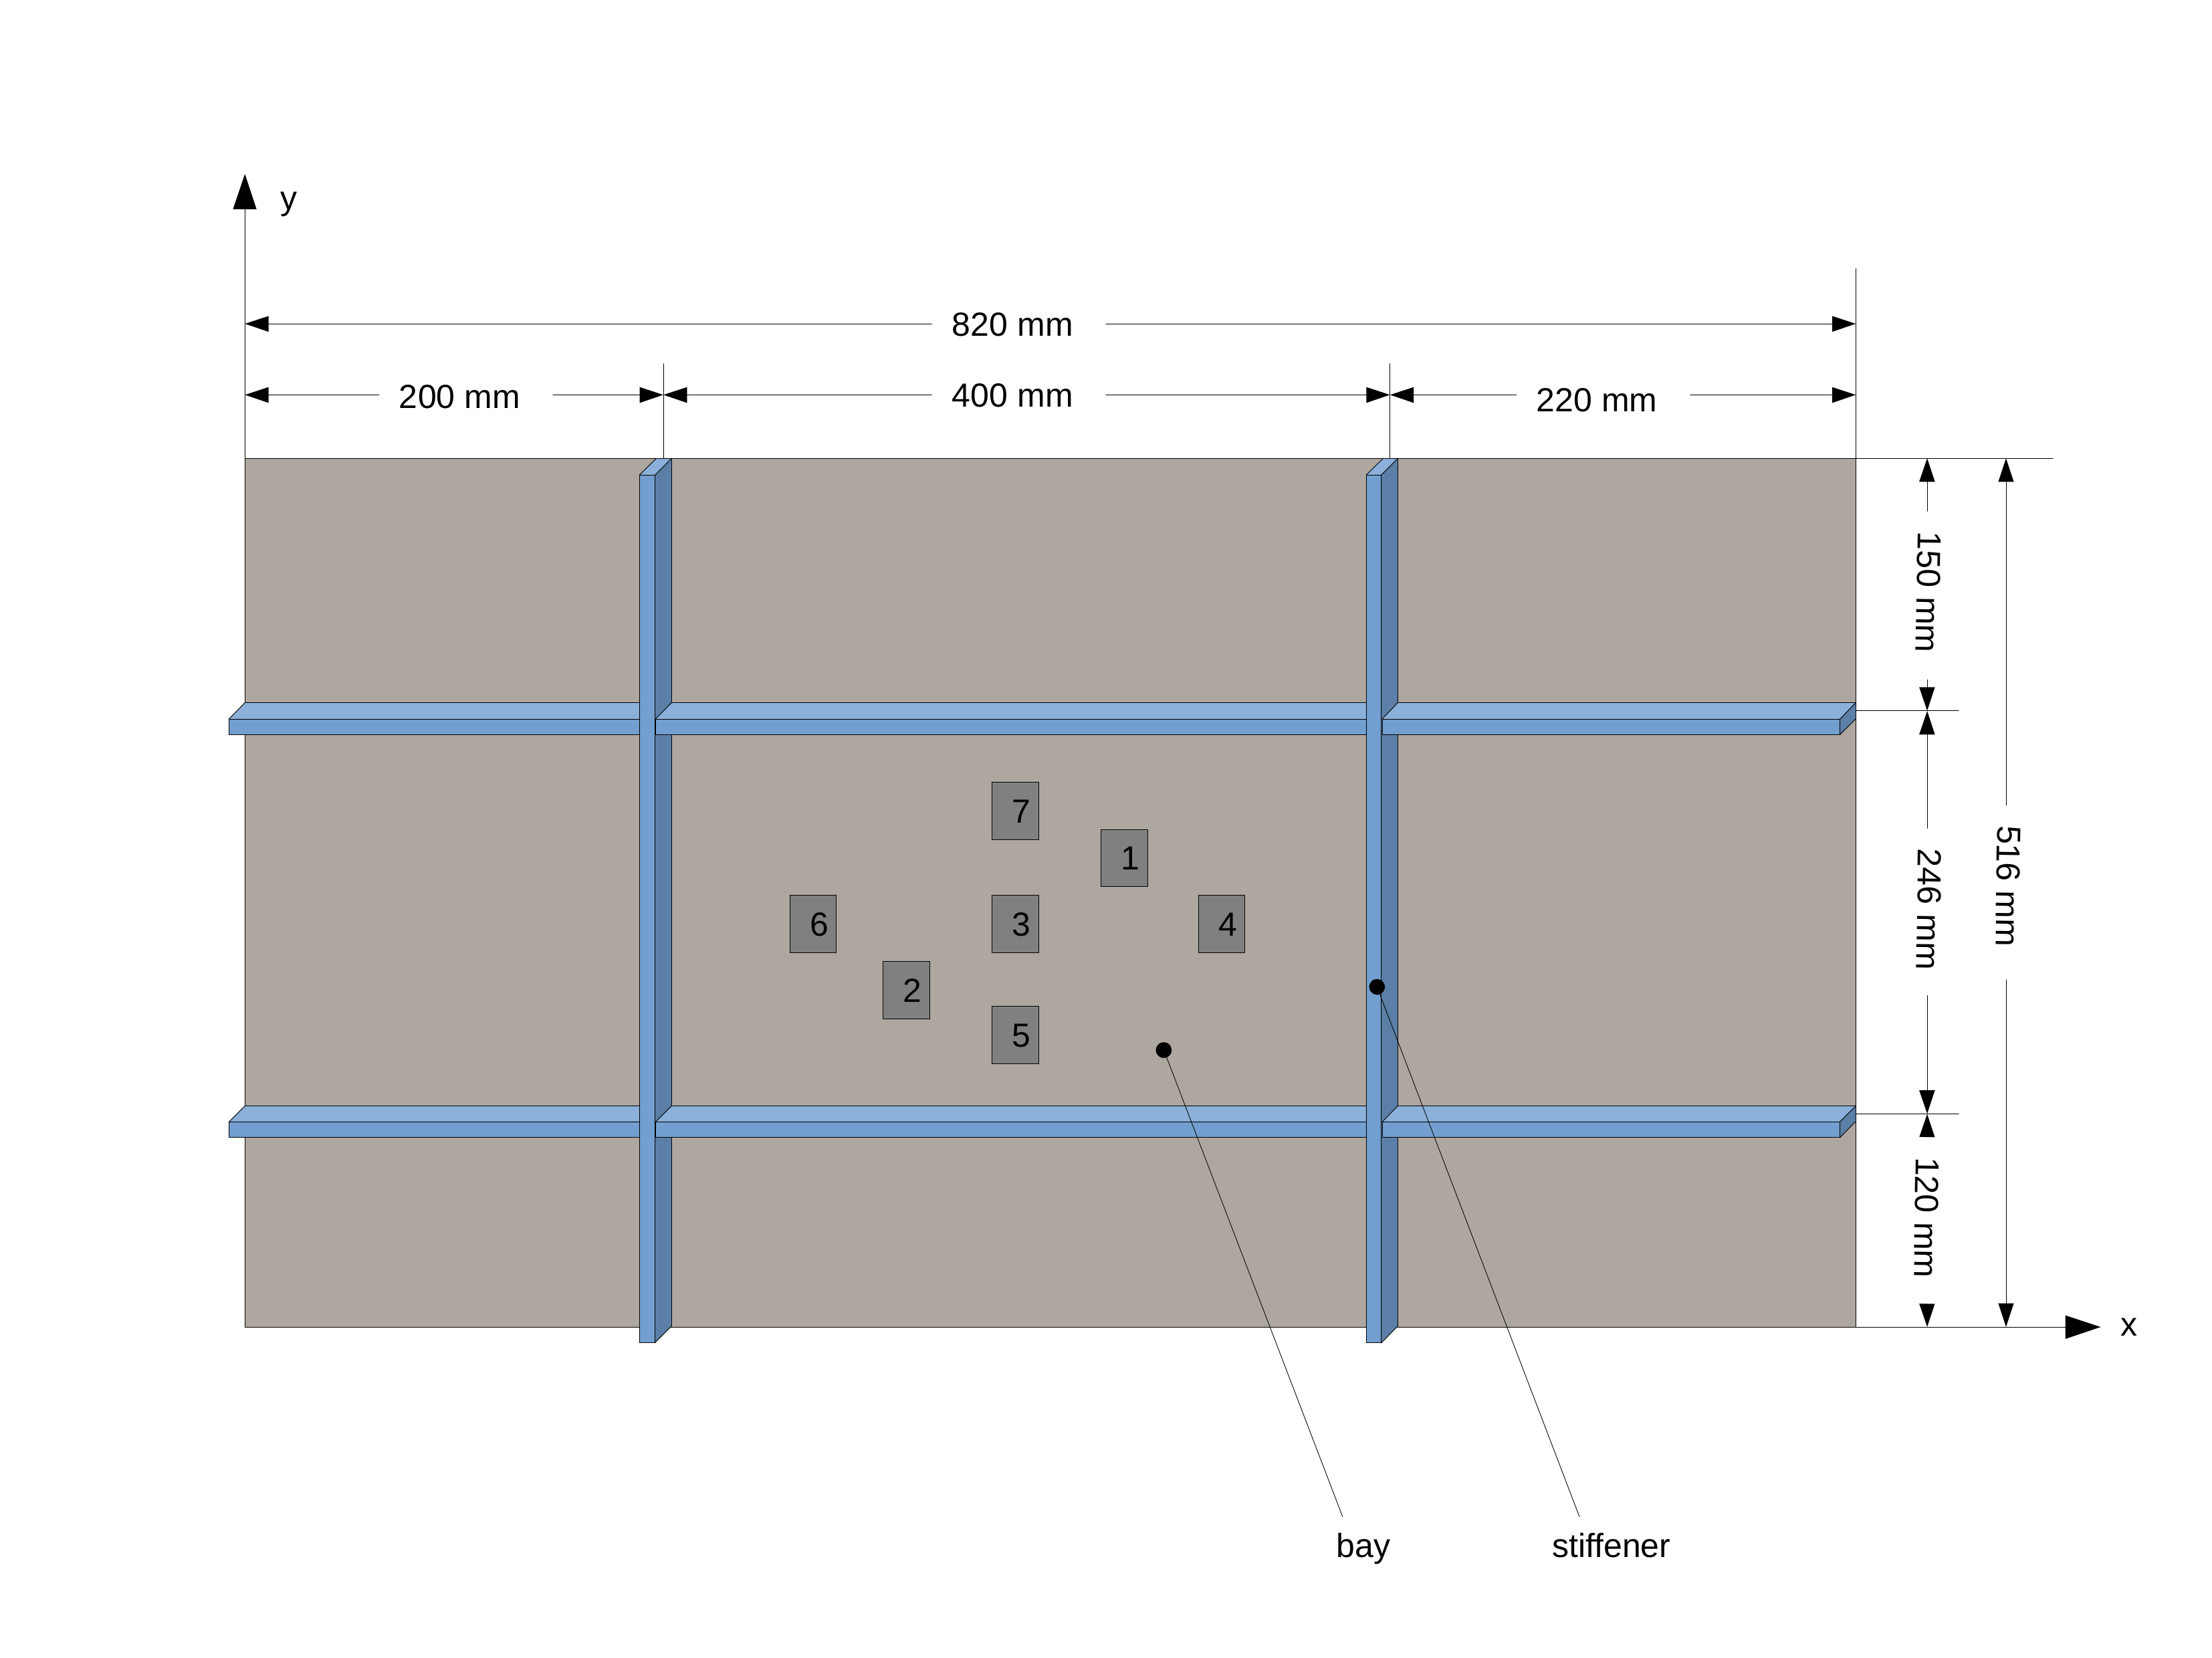
\includegraphics[trim = 2cm 1cm 0cm 2cm, clip, width=0.65\textwidth]{fig11.png}
  \caption{Scheme of the vibrating aircraft panel.}
  \label{fig:fig11}
  \end{figure}
 
 
 In order to verify the handling of higher dimensional systems, we apply our method to the vibration
 control of an aircraft panel. This example, taken from \cite{ji2014semi}, consists in 
 stabilizing the panel as close as possible to the equilibrium, which corresponds to 
 a null displacement inside the whole panel. In this purpose, 
 seven piezoelectric patches are glued on the panel, one is used for exciting the panel (patch 1 of Figure \ref{fig:fig11}),
 one is used as a sensor to evaluate the performance of the control (patch 2), one is used for the 
 observation of modal states (patch 6), and three are used for vibration control (patches 3 to 5), the last patch being
 used to validate the reconstruction (patch 7). For the numerical simulations, we choose the measurements 
 of the sensor patch as the output of the system. 
 
 Just as the cantilever beam, we use a finite element model reduced by modal decomposition
 then balanced truncation. The system is written exactly in the same way, 
 but with shell elements, and thus six degrees of freedom by node.
 The finite shell element model consists of $57000$ degrees 
 of freedom. We retain $50$ modes for the modal decomposition, and the model is reduced down to 
 $n_r = 5$ by balanced truncation. 
 Seven control modes are used for vibration control, it corresponds to a null voltage applied 
 on all the control patches, a positive constant voltage applied on each control patch
  (one patch is subject to a voltage at a time), and a negative
 constant voltage applied on each control patch. The reader is referred to \cite{ji2014semi} for more
 information on the exact functioning of the piezoelectric patches used in this
 case study, and see for example \cite{hagood1991,moheimani2006} for more general information
 on piezoelectric patches and their use for structural damping.
 With the same hardware configuration as in the previous example, the computation 
 of a decomposition took nearly a week. A simulation of the online procedure 
 is given in Figure \ref{fig:fig12} and \ref{fig:fig13}. 
 

 \begin{figure}[ht]
  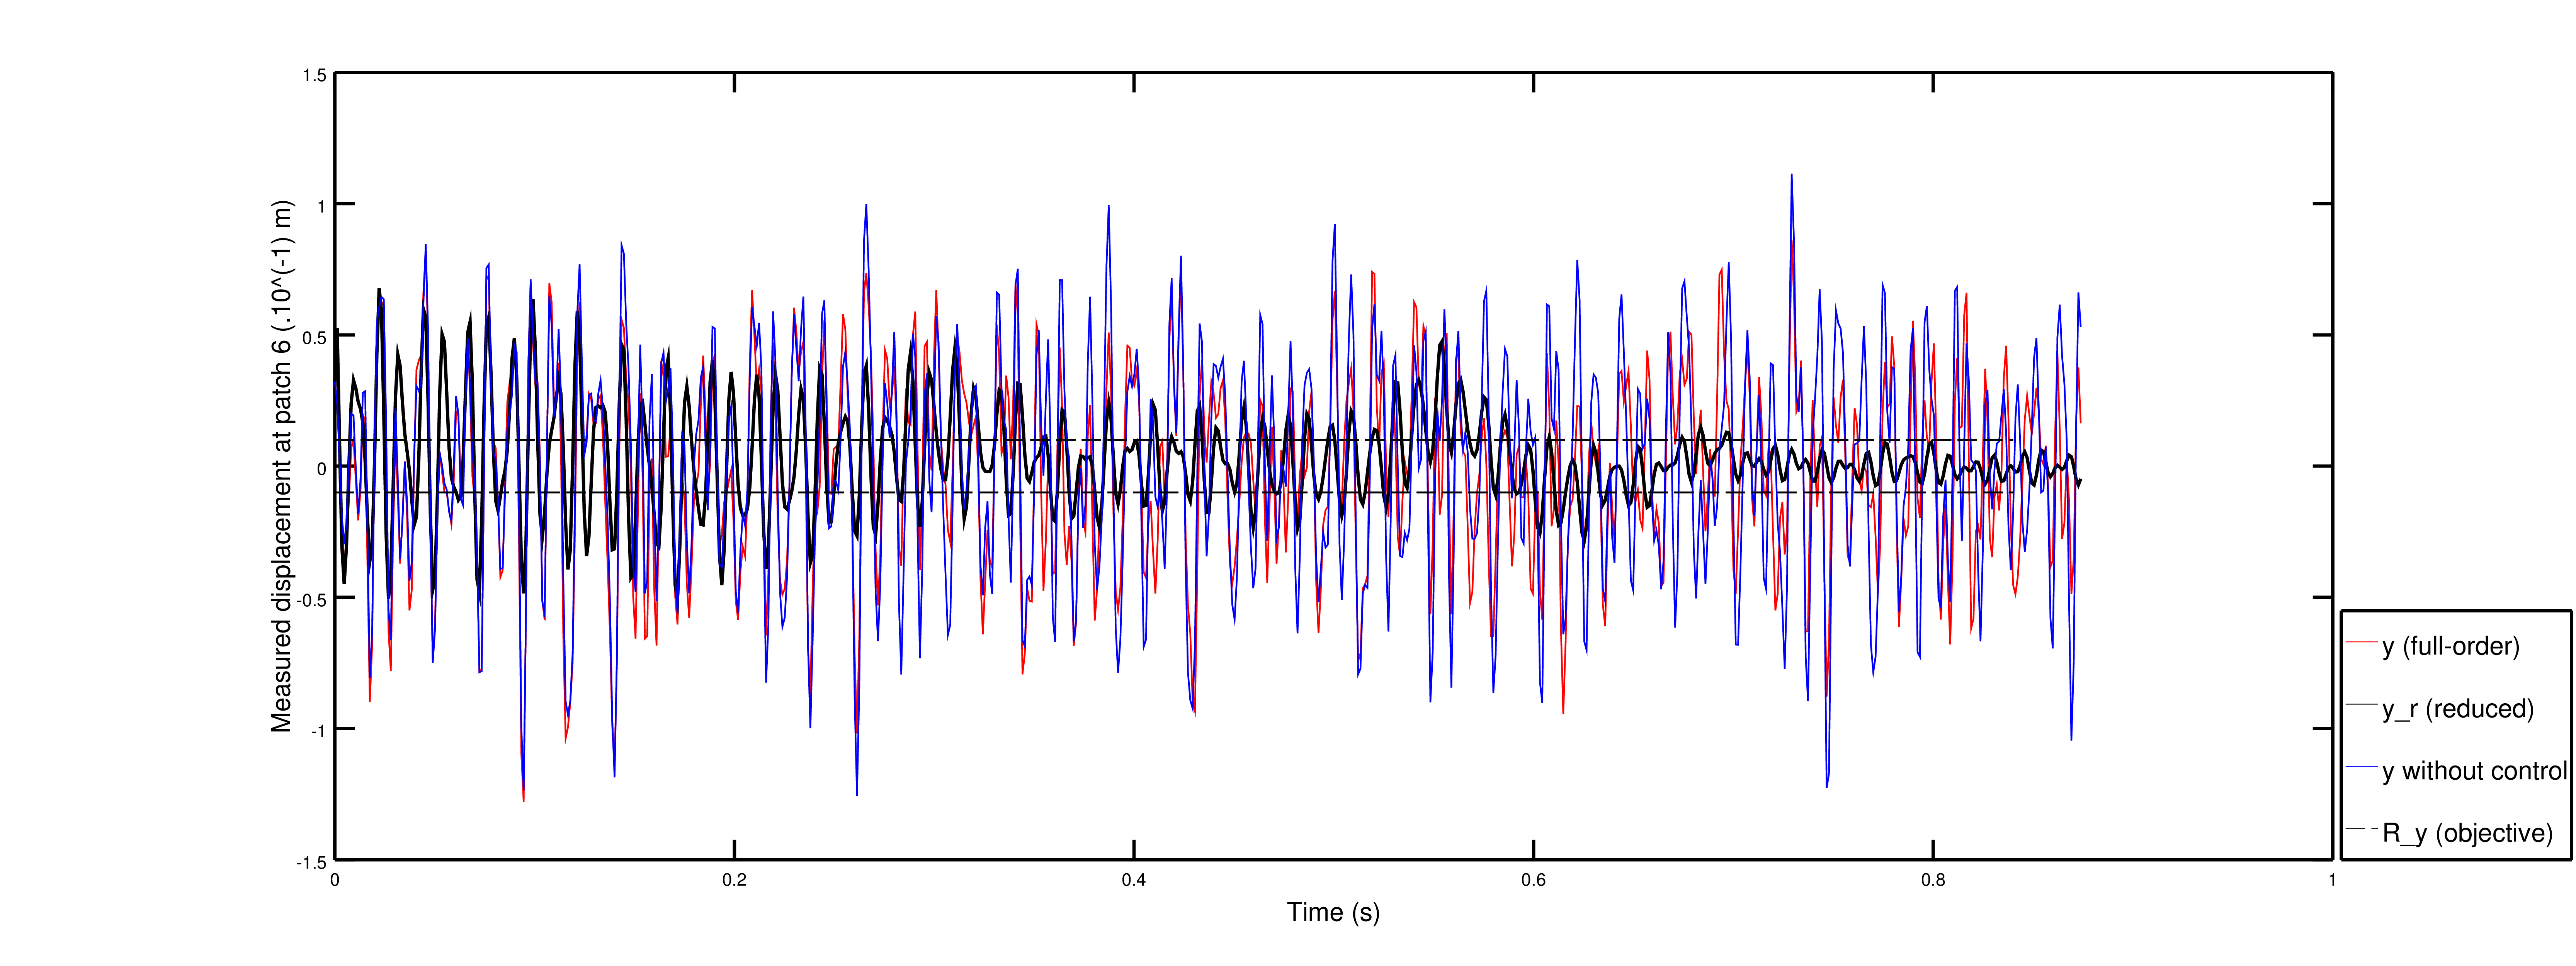
\includegraphics[trim = 3cm 0cm 0cm 1cm,clip, width=0.98\textwidth]{fig12.png}
  \caption{Simulation of vibration control of the aircraft panel.}
  \label{fig:fig12}
 \end{figure}
 
   \begin{figure}
   \centering
  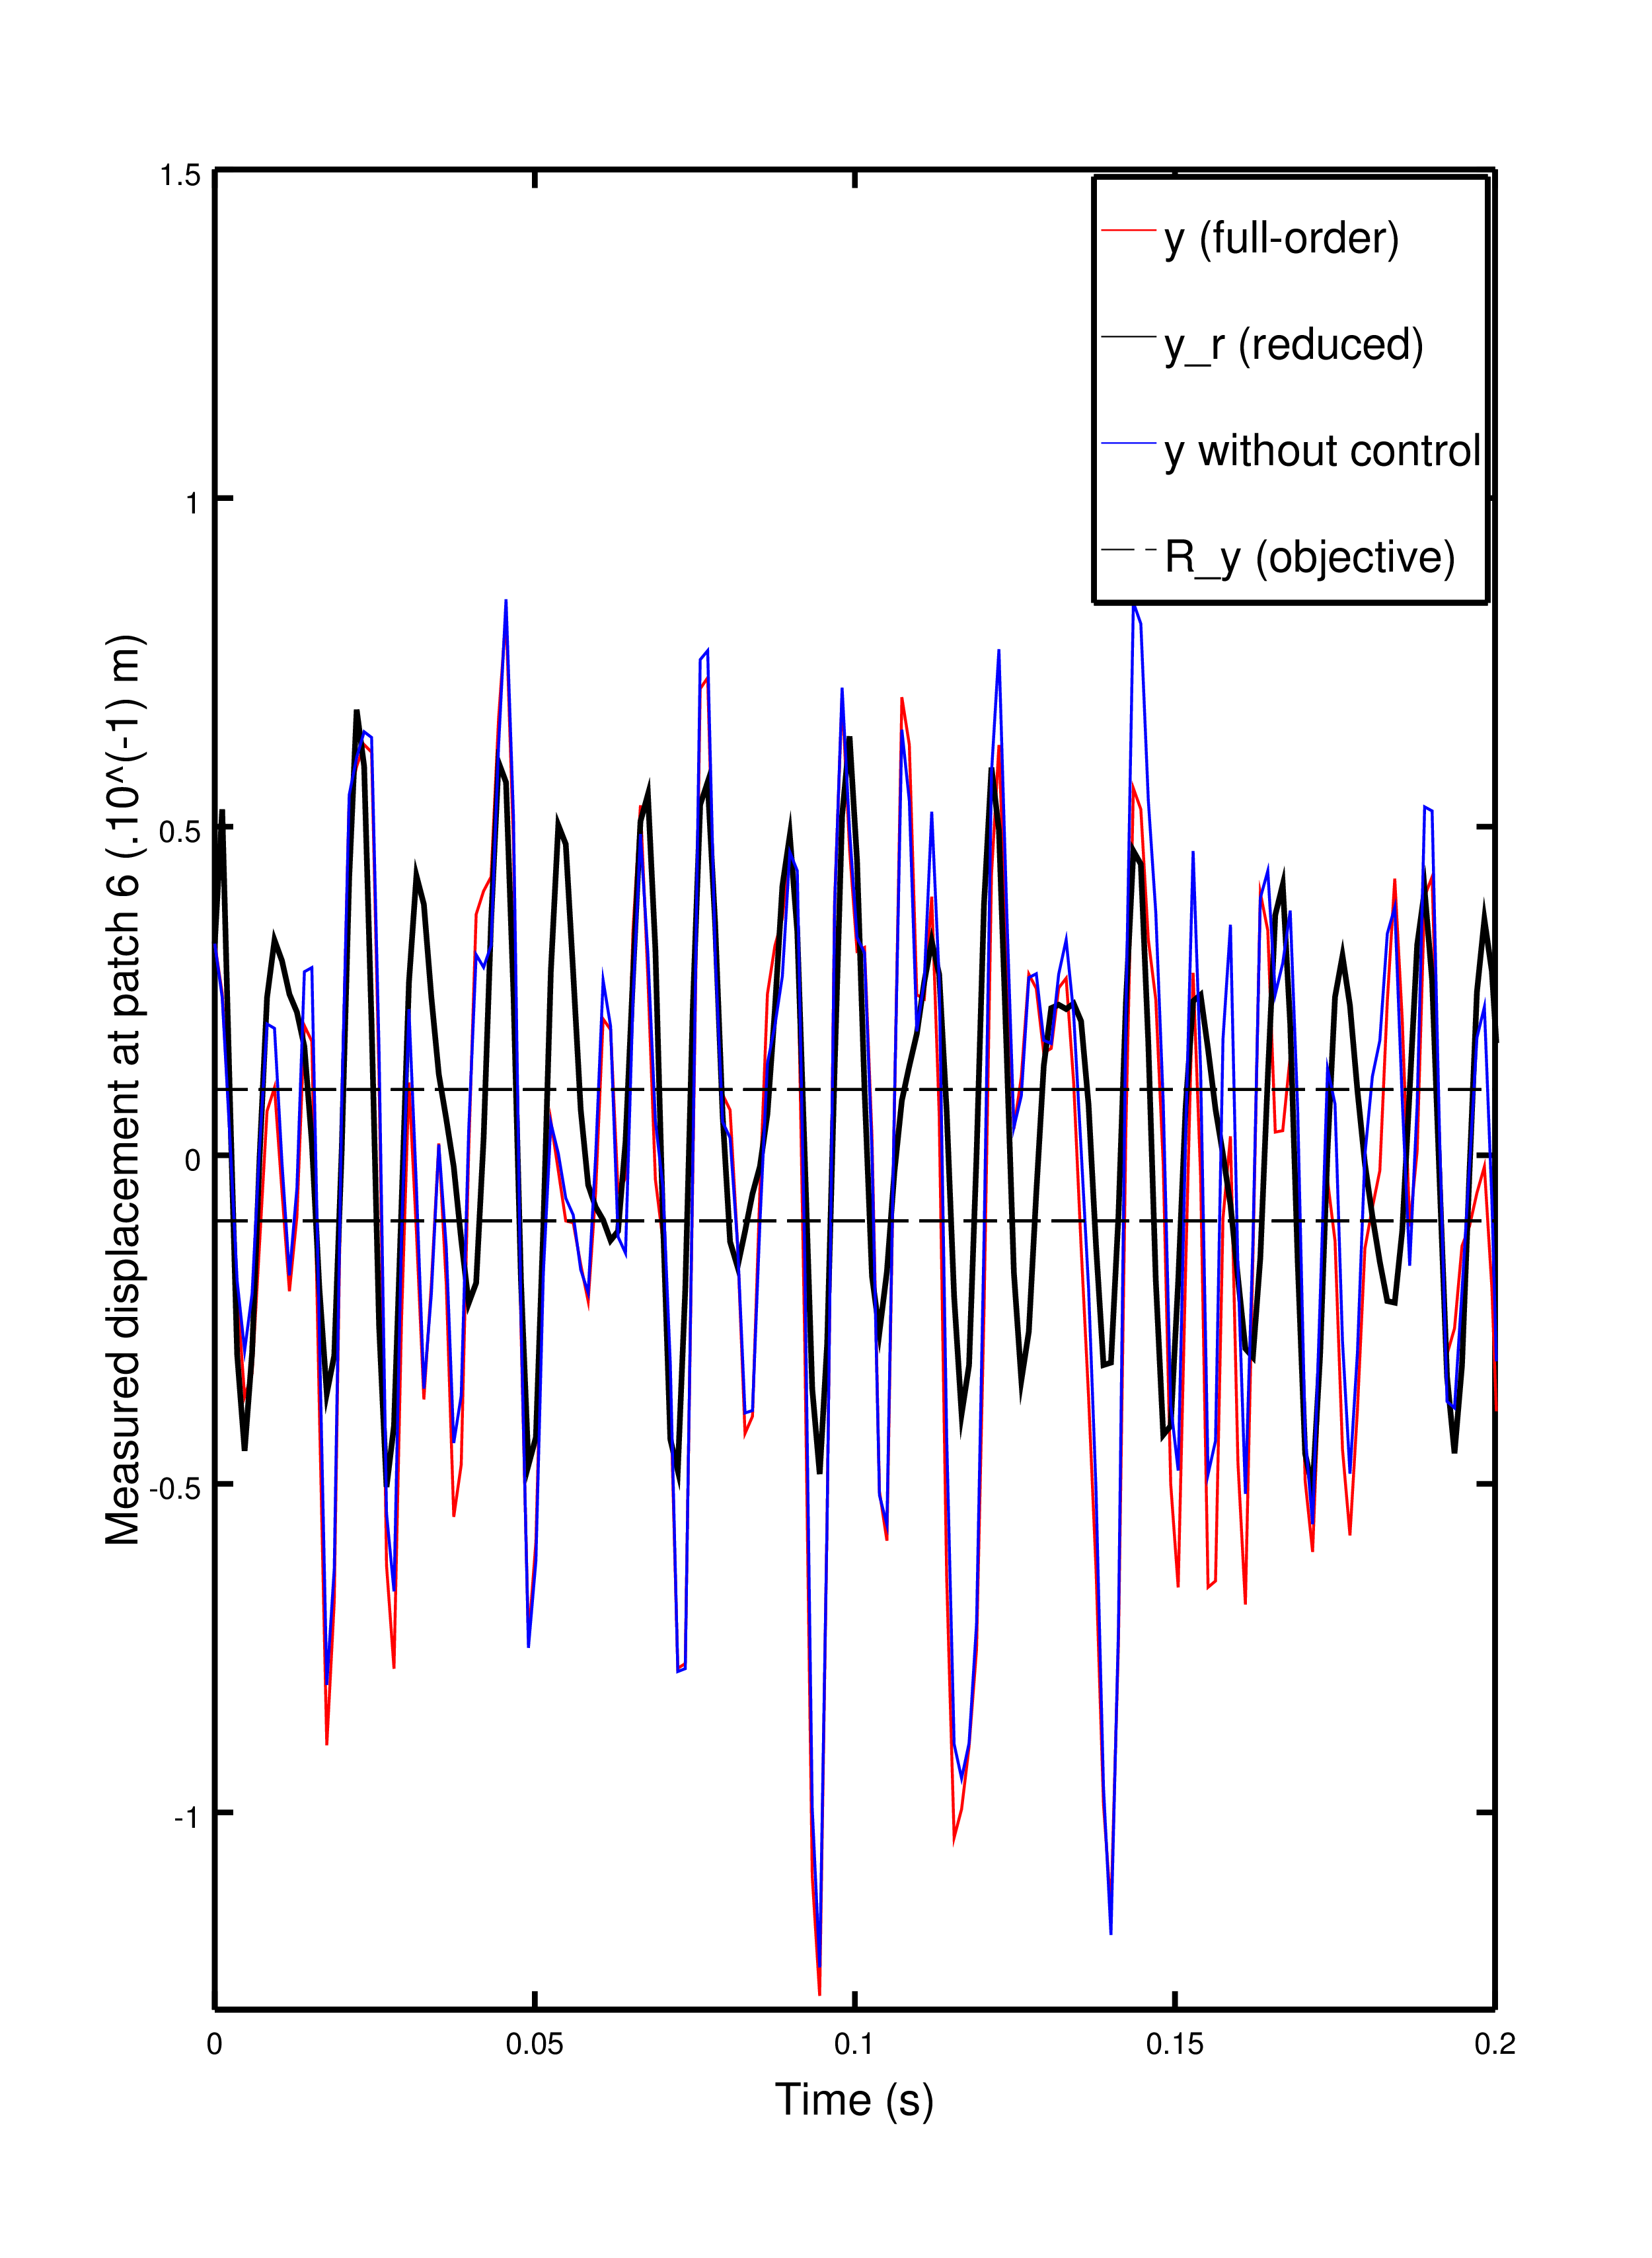
\includegraphics[width=0.55\textwidth]{fig13.png}
  \caption{Enlargement of Figure \ref{fig:fig13} on the time interval~$\lbrack 0,0.2 \rbrack$.}
  \label{fig:fig13}
 \end{figure}
 We observe that the response of the controlled full-order system is better than the non-controlled
 one, the main peaks observed in the non-controlled response are avoided. Nevertheless,
 the stabilization is not as efficient as one may expect. One can see that the reduced-order
 system is however well stabilized. This points out that the model reduction does not
 catch, in this case, all the information needed for control purposes. While we are currently 
 investigating new model reduction techniques, adapted to hyperbolic and non-linear systems, 
 we also think that in practice, the stabilization would be better because of the
 smoothness appearing in the applied torques in a real application.
 
 
 

  \section{Extension to Output Feedback Control}
  \label{sec:observation}
  
 So far, we designed reduced state-dependent controllers for switched control systems, permitting to 
 stabilize the output of the system in a given objective set $R_y$. During a real online use, one 
 is only supposed to know a part of the state of the system, such as measurements of sensors.
 We now want to take these partial measurements into account, by adding an intermediate step in the
 online use, namely, observation. We suppose that only the output of the system is known online.
 In the next sub-section, we introduce the principle of observation and give some preliminary
 results justifying the use of observers for switched control systems, allowing us to adapt our 
 algorithms to the use of observers. We then present some numerical results of the use of observers 
 with model order reduction. The whole approach with model order reduction is schemed in
 Figure \ref{fig:fig14}, but as we do not have any proof for the efficiency of the
 use of observers with model order reduction, we only provide some numerical simulations. 
 We are currently working on the establishment an error bound taking into account the projection error
 and the observation error, that will permit to construct a guaranteed reduced observer based control.
  
\subsection{Partial observation}

\begin{figure}
 \centering
 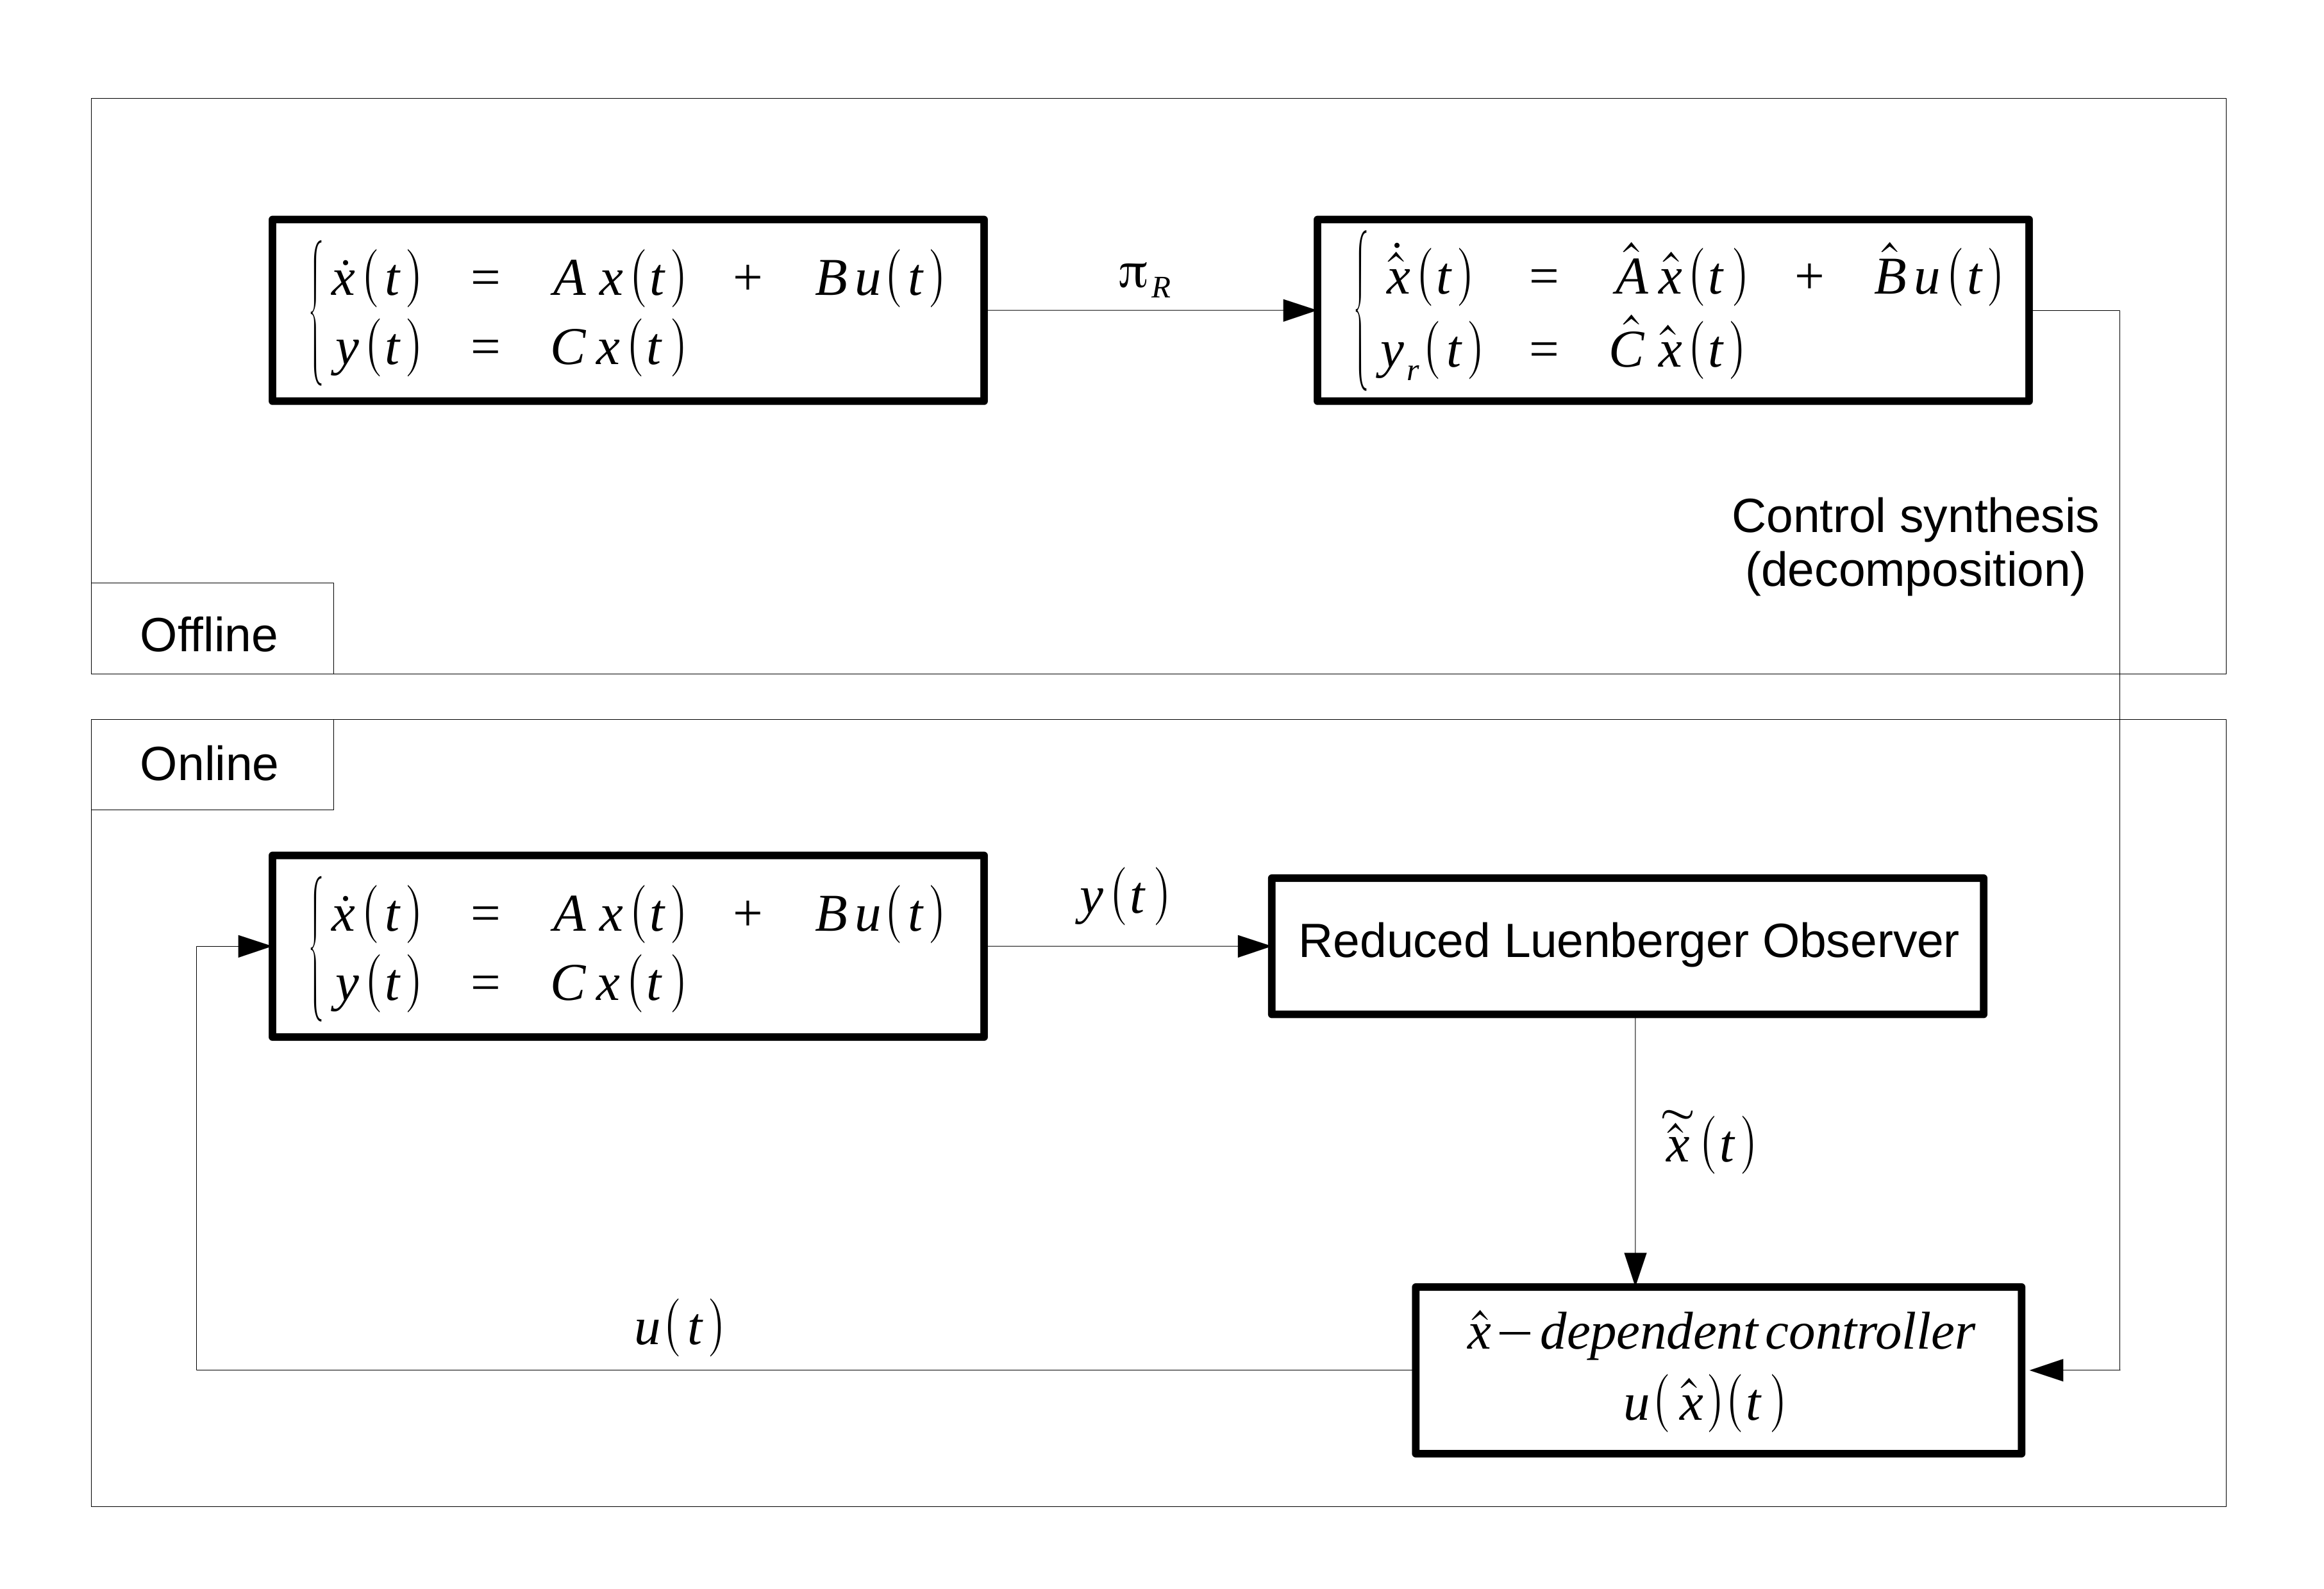
\includegraphics[width=0.7\textwidth]{fig14.png}
 \caption{Principle of the output feedback control}
 \label{fig:fig14}
\end{figure}


Having defined the state-space bisection algorithm for switched control systems
with output, we now add the constraint that the system is partially observed.
The objective is to design an {\em output feedback} 
controller using the state-space bisection algorithm introduced above. 


We recall that the switched system $\Sigma$ is written under the following form:
\begin{equation*}
 \Sigma : \left\lbrace
\begin{array}{ll}
\dot x(t) & =A x(t)+B u(t), \\
 y(t) & =C x(t).
\end{array}
\right.
\end{equation*}

We suppose that during an online use, one is only supposed to know $y(t)$ (we suppose
that $y$ can be measured in real time, that is at every time $t$).
If just this partial information of the state is known, we cannot directly 
apply our state-dependent controller synthesis method. An intermediate 
step must be introduced: the reconstruction of the state. The reconstruction is made 
with the help of an observer: it is an intermediate system that provides 
an estimate of the state of the system $\Sigma$ from the measurements of the output $y$ and the 
input $u$ of the system $\Sigma$. In fact, this means that we want
to design an output feedback law for the system $\Sigma$ with the help of an observer.
In this paper, we retain the Luenberger observer \cite{ELO1987,alessandri2001,alessandri2007luenberger}
to reconstruct the 
state of $\Sigma$, it is subject to the following equation:
\begin{equation}
 \dot {\tilde x} = A \tilde x - L(u)(C \tilde x - y) + Bu, \quad L(u) \in \mathbb{R}^{n\times m}
\label{eq:luenberger}
 \end{equation}

Obviously, the observer does not reconstruct exactly the state $x$ of the system $\Sigma$, 
we thus introduce the reconstruction error $\eta(t) = \Vert x(t) - \tilde x(t) \Vert $.
Our goal is to control the system $\Sigma$ with this estimate $\tilde x$: we apply 
a law $u(\tilde x)$. One can note that the method relies on the convergence
of the observer $\tilde x$ to the state $x$, this aspect is developed in the following section.

The entries of the control problem we retain are then the following:
\begin{itemize}
 \item an interest set $R_x \subset \mathbb{R}^n$,
 \item an objective set $R_y \subset \mathbb{R}^m$,
 \item an initial, a priori known, reconstruction error $\eta_0$.
\end{itemize}

With the method given below, the 
outputs of the problem are the following:
\begin{itemize}
  \item a decomposition of $R_x$ w.r.t. $\eta_0$ and the dynamics of $\Sigma$,
  \item a procedure to  choose $u$ knowing $\tilde x$,
  \item and the guarantee that, for any pattern $Pat$, if $x_0 \in R_x$ and $\eta(0) \leq \eta_0$, then \newline 
  $ {\bf x}(\vert Pat \vert \tau,x_0,Pat) \in R_x$ and
  ${\bf y}(\vert Pat \vert \tau,x_0,Pat) \in R_y$.
 \end{itemize}

Let us now introduce some hypotheses and important results to ensure the 
efficiency of the method.


\subsection{Convergence of the observer}


The properties of the  Luenberger observer  depend on the choice of the 
matrices $L(u)$ appearing in \eqref{eq:luenberger}. 
A crucial assumption in what follows is that 
it is possible to choose $L(\cdot)$ in such a way that
the modes of the Luenberger observer 
share a common non-strict quadratic Lyapunov functions, i.e., there exists 
a positive definite matrix $P$ such that:
\begin{equation}\label{w-Lyapunov}
\forall u, \quad P (A + L(u)C) + (A + L(u)C)^\top P \leq 0.
\end{equation}


The dynamics of the original switched system and of the Luenberger switch observer
can be grouped in the  augmented system
\[
\left(
\begin{array}{l}
\dot{\tilde x } \\
 \dot x
\end{array} \right) = 
\left( \begin{matrix}
A-L(u)C & L(u)C \\
 0 & A
\end{matrix} \right) \left( \begin{array}{l}
                            \tilde x \\ x 
                           \end{array} \right)
                            + \left( \begin{array}{l}
                               Bu \\ Bu
                              \end{array} \right).
\]

Define $e(t)=  x(t) - \tilde x(t)$ and  $\eta(t)= e(t)^T P e(t)$. By definition $e(\cdot)$ satisfies 
\begin{equation}\label{eq:augmented_sys}
\dot e= (A-L(u)C)e
\label{eq:e}
\end{equation}
and assumption \eqref{w-Lyapunov} implies that $\eta$ is non-increasing along all trajectories.
The patterns in $u(\cdot)$ will be chosen in order to guarantee that not only $\eta$ decreases, but actually converges to zero. 



An assumption which may be motivated by the technical constraints of the system under consideration
is the existence of a \emph{dwell-time}, that is, a positive constant $\tau$ such that two subsequent
discontinuities of $u(\cdot)$ have a distance of at least $\tau$ (recall that $u(\cdot)$ is assumed to 
be piecewise constant). 
The dwell-time condition not only reflects technological constraints, 
but is also useful in the asymptotic analysis of the switched system (\ref{eq:LTI}). 
The basic result that we will use is a simplified version of 
\cite[Theorem II.5]{serres2011convergence}, which states that under the dwell-time hypothesis,
and by choosing properly the patterns, one can manage to make $\eta(t)$
converge to $0$.
(For further asymptotic results of linear switched systems with a common non-strict 
quadratic Lyapunov function, see \cite{Moussa-Jouan2011,Riedinger-Sigalotti-Daafouz2010}.)


The strategy suggested by the previous theorem is the following: 
\begin{itemize}
\item identify $u_{*,1},\dots,u_{*,m}$ such that 
\[ \cap_{j=1}^m \mathrm{Ker}(A-L(u_{*,j})C)=(0); \]
\item impose that each pattern takes all values $u_{*,1}$, $\dots$, $u_{*,m}$.
\end{itemize}

Under these constraints the solution $e$ of \eqref{eq:e} is guaranteed to converge to the origin (monotonically with respect to the norm induced by the positive matrix $P$). 



In the case of the metal plate we will see that it is sufficient to take $m=2$ and that 
the constraint that each pattern passes trough the two values $u_{*,1},u_{*,2}$ is 
not a heavy obstacle in the implementation of the proposed algorithm. 
As a result, we will obtain a strategy $u(\tilde x)$ that, under the assumption that the
initial state $x(0)$ and the initial estimation $\tilde x(0)$ are in $R_x$
and satisfy $\eta(0)<\eta_0$, the trajectory 
${\bf x}(t,x(0),u)$ and the estimated trajectory, denoted by ${\bf \tilde x}(t,\tilde x(0),u)$, are 
such that the evaluation of ${\bf x}(\cdot)$ after each pattern is again in $R_x$ and 
${\bf x}(t,x(0),u)- {\bf \tilde x}(t,x(0),u)\to 0$ as $t\to+\infty$. 

\subsection{Observer based decomposition}

We present here the adaptations of the algorithms taking the observation into account.
The {\em observer based decomposition} algorithm takes $\eta_0$ as a new input.
Given a system $\Sigma$, two sets $R_x \subset \mathbb{R}^n$ and
$R_y \subset \mathbb{R}^m$,
a positive integer $k$, and an initial reconstruction error $\eta_0$, a  
successful observer based decomposition
returns a set $ \tilde \Delta$
of the form $\{V_i,Pat_i\}_{i \in I}$, where~$I$ is a finite set of indices, every $V_i$ 
is a subset of~$R_x$, and every $Pat_i$ is a $k$-pattern such that:
\begin{itemize}
\item[(a)] $\bigcup_{i \in I}V_i = R_x$,
\item[(b)] for all $i \in I$: $Post_{Pat_i}(V_i + \eta_0) \subseteq R_x - \eta_0$,
\item[(c)] for all $i \in I$: $Post_{Pat_i,C}(V_i + \eta_0) \subseteq R_y$.
\end{itemize}




Such a decomposition allows to perform an output feedback control on $\Sigma$ as 
stated in the following.
The algorithm relies on two functions given in 
Algorithms \ref{alg:decompo_obs} and \ref{alg:findPat_obs}.
If a successful observer based decomposition is obtained, it naturally induces an
estimate-dependent control, which we denote by $\mathbf{u}_{\tilde \Delta}$.
By looking for patterns mapping $R_x + \eta_0$ into $R_x$, we guarantee that 
${\bf x}(t,x,u)$ is stabilized in $R_x$. 
Indeed, if $x(0)$ is the initial state, and $\tilde x(0)$ the initial estimation (supposed belonging to
$R_x$), we know that $\tilde x(0)$ belongs to $V_{i_0}$ for some $i_0 \in I$, 
and that $x(0)$ belongs to $V_{i_0}+\eta_0$,
so the application of the pattern $Pat_{i_0}$ yields ${\bf x}(\vert Pat_{i_0} \vert \tau,x(0),Pat_{i_0}) \in R_x -\eta_0$ (because $Post_{Pat_{i_0}}(V_{i_0} + \eta_0) \subseteq R_x -\eta_0$)
and ${\bf \tilde x}(\vert Pat_{i_0} \vert \tau,\tilde x(0),Pat_{i_0}) \in R_x$ because 
\[\begin{aligned} \Vert {\bf x}(\vert Pat_{i_0} \vert \tau,x(0),Pat_{i_0}) - {\bf \tilde x}(\vert Pat_{i_0} \vert \tau,\tilde x(0),Pat_{i_0}) \Vert & \\ < \eta_0.& \end{aligned}\]
Note that we plan to improve these algorithms by taking the decrease of $\eta(t)$ into account, 
so that the decomposition is less restrictive when $\eta(t)$ is small.

\begin{algorithm}[!ht]
\centering
\begin{algorithmic}

 \STATE{{\bf Input:} A box $W$, a box $R_x$, a box $R_y$, a degree $D$ of bisection, 
a length $K$ of input pattern, an initial reconstruction error $\eta_0$}
  \STATE{{\bf Output:} $\langle\{(V_i,Pat_i)\}_{i},True\rangle$ with $\bigcup_i V_i=W$,
$\bigcup_i Post_{Pat_i}(V_i + \eta_0)\subseteq R_x$ and $\bigcup_i Post_{Pat_i,C}(V_i + \eta_0)\subseteq R_y$ ,  %and $\bigcup_i Unf_{Pat_i}(V_i)\subseteq S$
or $\langle\_ ,False\rangle$}
  \STATE{$(Pat,b) := Find\_Pattern(W,R_x,R_y,K,\eta_0)$}\\
  \IF{$b=True$}{
    \STATE{{\bf return} $\langle\{(W,Pat)\},True\rangle$}
  }
  \ELSE
      \IF{$D=0$}{
	  \STATE{{\bf return} $\langle\_ ,False\rangle$}
       }
       \ELSE \STATE{Divide equally $W$ into $(W_1,\dots, W_{2^{n}})$ }\ \ \ \\
	    \FOR{$i=1\dots2^{n}$} \STATE{
	      $(\Delta_i,b_i)$ := Decomposition\_Obs($W_i$,$R_x$,$R_y$,$D - 1$,$K$,$\eta_0$)\\
	    }
	    \ENDFOR  
 	      \STATE{{\bf return} $(\bigcup_{i=1\dots 2^{n}} \Delta_i,\bigwedge_{i=1\dots 2^{n}} b_i)$}
 	    
	\ENDIF	    
\ENDIF
\end{algorithmic}
\caption{\small Decomposition\_Obs($W,R_x,R_y,D,K,\eta_0$)}  
\label{alg:decompo_obs}  
\end{algorithm}

 \begin{algorithm}[!ht]
 \centering
 \begin{algorithmic}
 \STATE{{\bf Input:} A box $W$, a box $R_x$, a box $R_y$, a length $K$ of input pattern, an initial reconstruction error $\eta_0$}
 \STATE{{\bf Output:} $\langle Pat,True\rangle$ with $Post_{Pat}(W + \eta_0)\subseteq R_x$,$Post_{Pat,C}(W + \eta_0)\subseteq R_y$, or $\langle\_, False\rangle$ when 
no input pattern maps $W+\eta_0$ into $R_x$}
   \FOR{$i=1\dots K$} \STATE{$\Pi :=$ set of input patterns of length $i$}\\
    \WHILE{$\Pi$ is non empty} \STATE{Select $Pat$ in $\Pi$\\ $\Pi:= \Pi\setminus  \{Pat\}$}\\ \IF{$Post_{Pat}(W + \eta_0) \subseteq R_x - \eta_0$ and $Post_{Pat,c}(W + \eta_0) \subseteq R_y$  } 
    {\RETURN{$\langle Pat,True\rangle$}} 
    \ENDIF
    \ENDWHILE
    \ENDFOR
   \RETURN{$\langle\_ ,False\rangle$}
    \end{algorithmic}
 \caption{\small Find\_Pattern\_Obs($W,R_x,R_y,K,\eta_0$)}
\label{alg:findPat_obs}
 \end{algorithm}


\subsection{Reduced output feedback control}

Algorithms \ref{alg:decompo_obs} and \ref{alg:findPat_obs} allow to synthesize guaranteed output
feedback controllers for switched control systems without model order reduction.
However, the use of model order reduction and observation
for the thermal problem of section \ref{sec:thermal} is indeed possible, this is partly 
enabled thanks to the elliptic nature and highly contractive behavior of the system.

The online simulations are performed just as sated in Figure \ref{fig:fig14}.
From the full-order system $\Sigma$, we build a reduced-order system $\hat \Sigma$ by balanced
truncation. An $\varepsilon$-decomposition is then performed on $\hat \Sigma$, 
yielding a $\hat x$-dependent controller (the decomposition was obtained in
about two minutes). The control $u(\tilde{\hat x})$ is then computed online with the 
reconstructed variable $\tilde {\hat x}$, which dynamics is the following:
\begin{equation}
 \dot {\tilde {\hat x}} = \hat A \tilde {\hat x} - L(u)(\hat C \tilde{\hat x} - C x) + \hat B u, \quad L(u) \in \mathbb{R}^{n_r\times m}
\label{eq:luenberger_red}
 \end{equation}


As the $\varepsilon$-decomposition is
already quite restrictive (i.e. the error bound overestimates the real
projection error) and because the Luenberger observer converges fast,
we observe that the induced control already works, even if we do not have any 
justification of the efficiency yet. The proof should be established
by evaluating, for any pattern $Pat$, a bound of the following error:
\begin{equation}
   \Vert \pi_R {\bf x}(\vert Pat\vert \tau ,x(0),Pat) - {\bf {\tilde {\hat x}}}(\vert Pat\vert \tau ,\tilde {\hat x}(0),Pat) \Vert
 \label{eq:to_proof}
\end{equation}


In the simulations Figures \ref{fig:fig15} and \ref{fig:fig16}, the full-order system is 
of order $n=897$, the reduced order system of order $n_r = 2$. The full-order system
is initialized with a uniform temperature field of $x(0) = 0.06^{n}$. The reduced observer is initialized
at $\tilde{x}(0) = 0^2$.
The two projected variables $\pi_R x$ cannot be reconstructed exactly because of (at least) the
projection error, but the output is still very well reconstructed. 
Both the observer and the full-order outputs are sent in the objective set $R_y$, which means
that we should manage to control a thermal problem just with the information
obtained with few sensors.

\begin{figure}
 \centering
 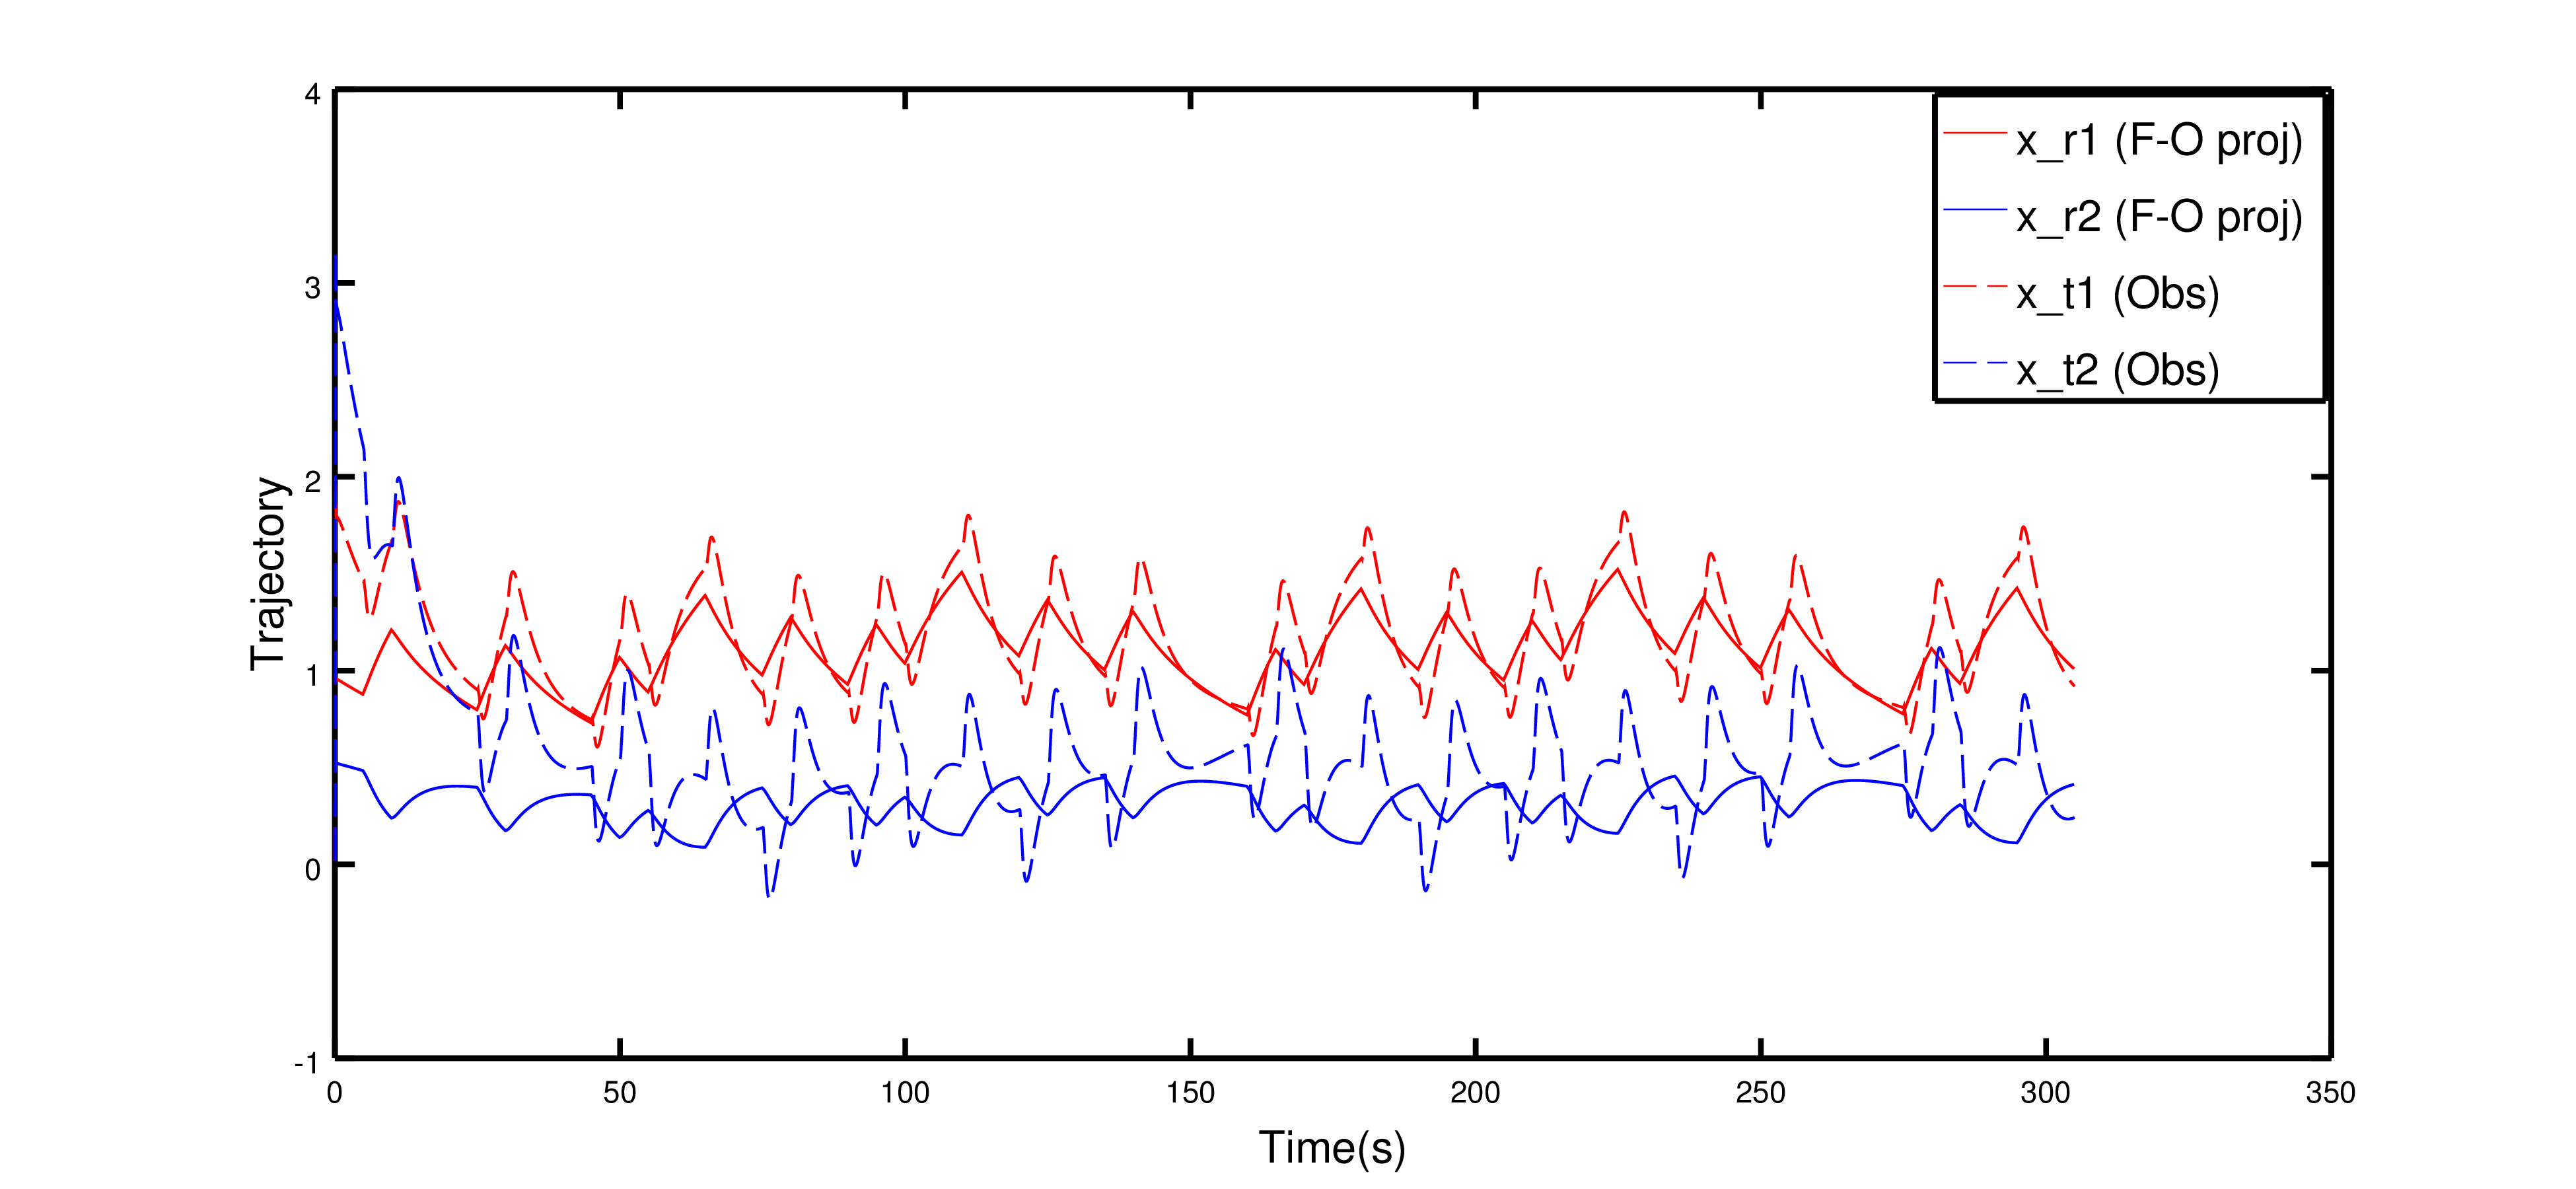
\includegraphics[width=129mm]{fig15.png}
 \caption{Simulation of the thermal problem with observation: projected variables. $x$\_$r1$ and $x$\_$r2$
  are the two variables $\pi_R x$ plotted within time (plain lines), it corresponds to
 the projection of the full-order system state. $x$\_$t1$ and $x$\_$t2$ are
 the two variables $\tilde{\hat x}$ plotted within time (dotted lines), it corresponds to
 the state of the reduced observer.}
 \label{fig:fig15}
\end{figure}

\begin{figure}
 \centering
 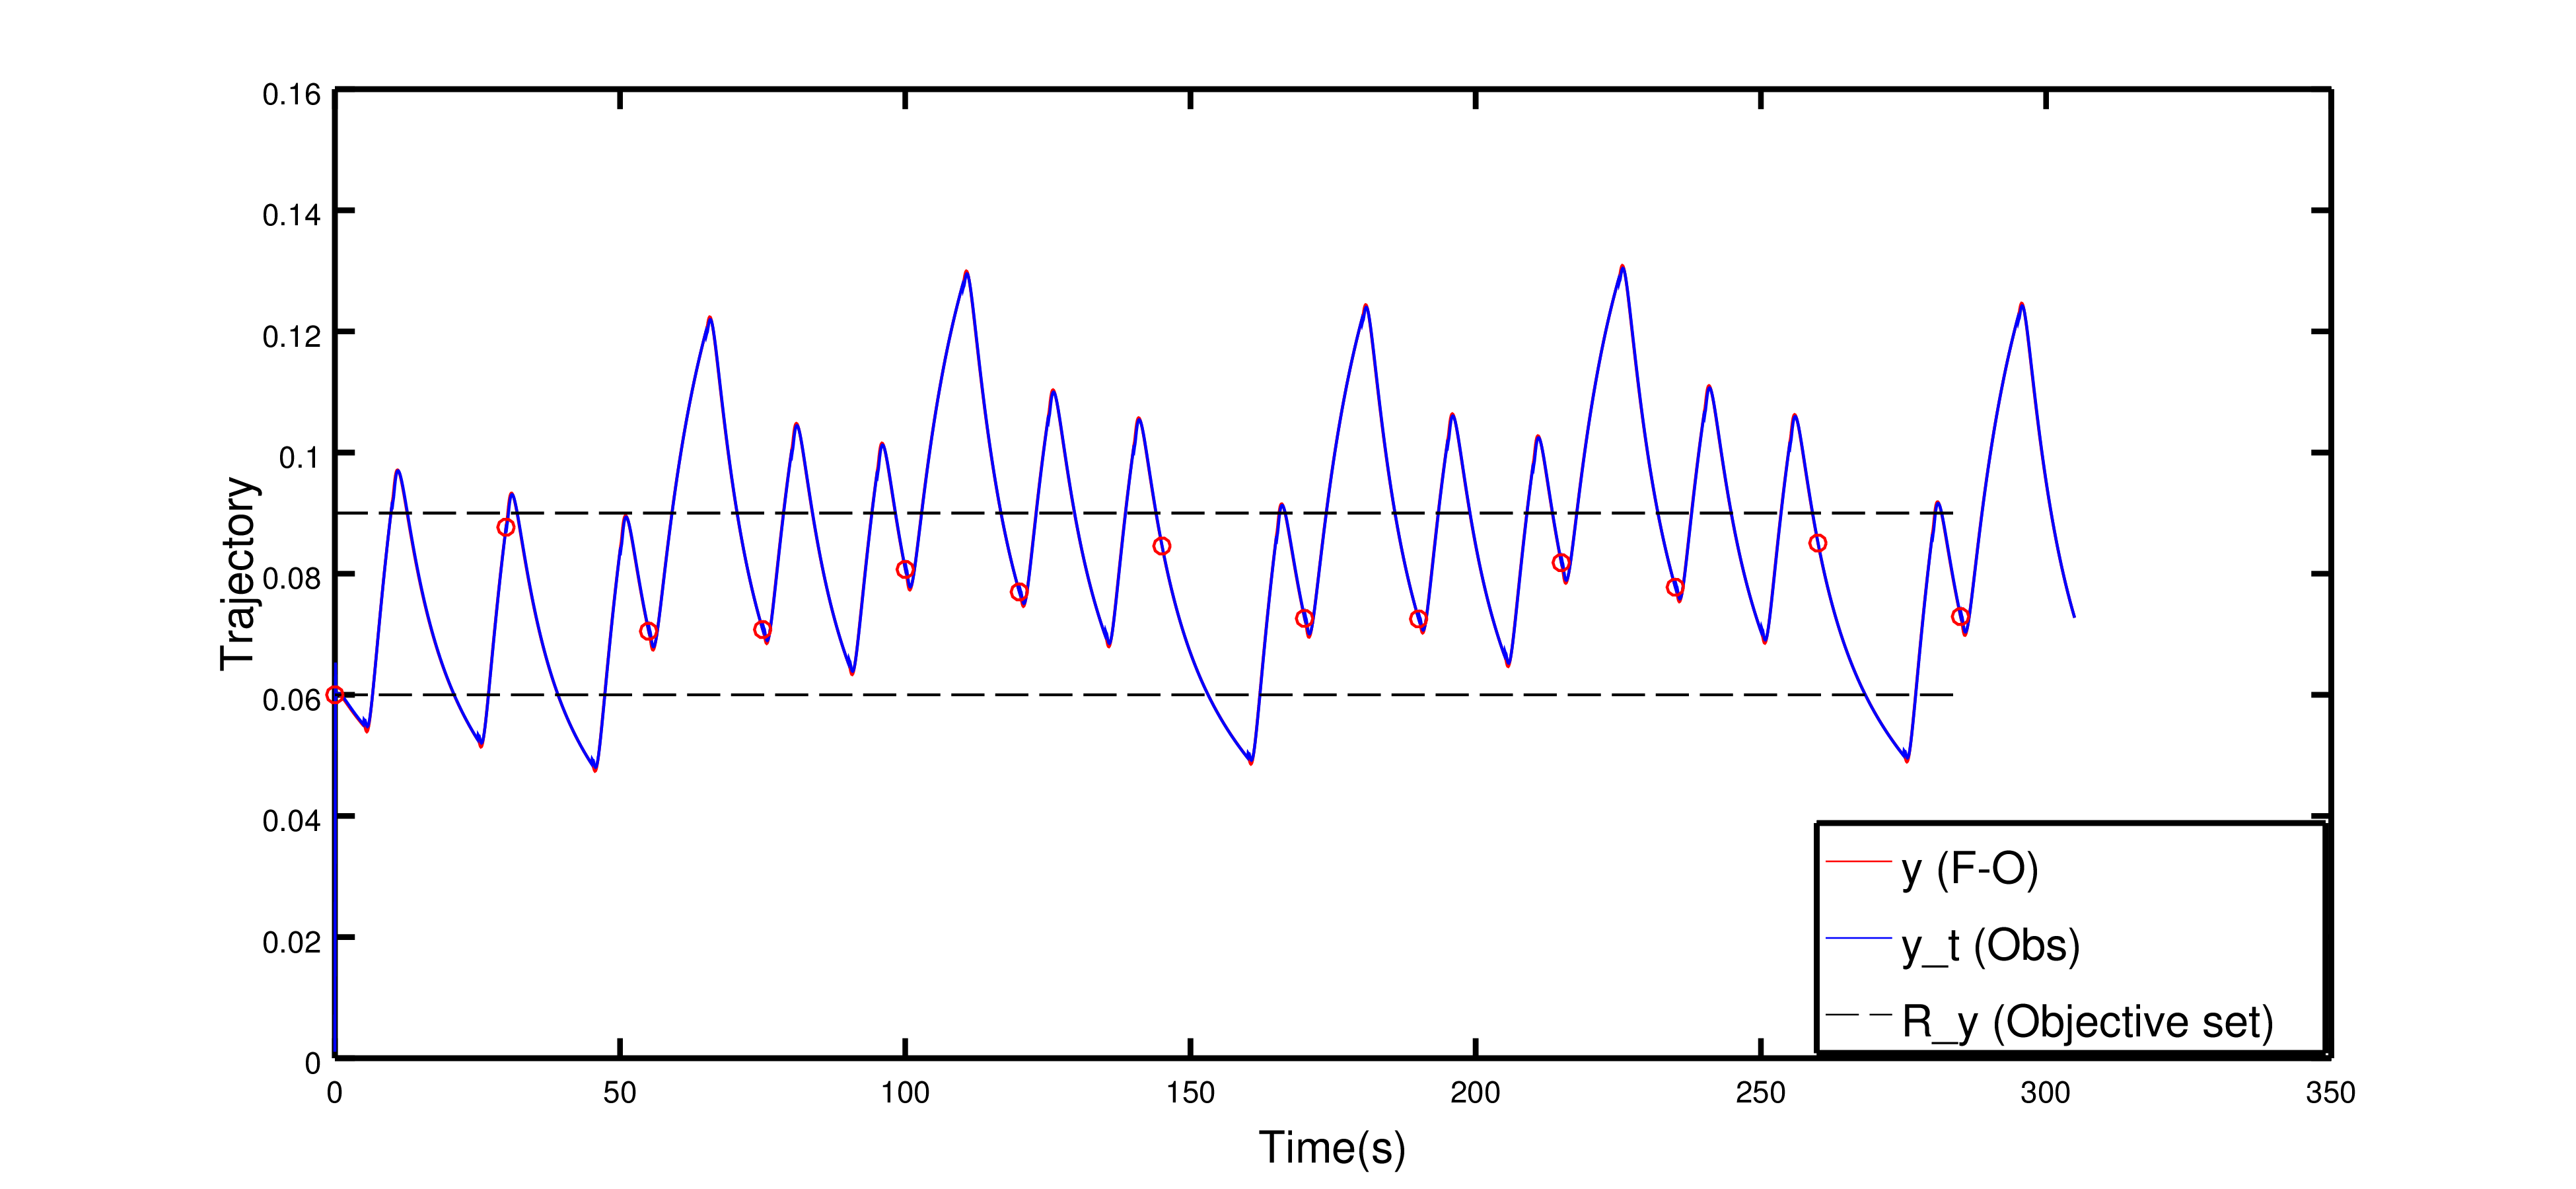
\includegraphics[width=129mm]{fig16.png}
 \caption{Simulation of the thermal problem with observation: output variables. The output 
 of the full-order system (plain red) coincides with the output reconstructed by the observer (plain blue),
both are sent in the objective set at the end of patterns (red circles).}
 \label{fig:fig16}
\end{figure}


 \section{Final Remarks}
 \label{sec:conclusion}
Two methods have been proposed to synthesize controllers for switched control systems using
model order reduction and the state-space bisection procedure. 
An offline and an online use 
are enabled, both uses are efficient but they present different advantages.
The offline method allows to obtain the same behavior as the reduced-order model, but 
the associated bound is more pessimistic, and the controller has to be computed before the
use of the real system. The online method leads to less pessimistic bounds but implies
a behavior slightly different from the reduced-order model, and the limit cycles may be different
from those computed on the reduced system.
The behavior of the full-order system is thus less known, but its use can be performed 
in real time.

A first step to the online reconstruction of the state of the system has been done
with the help of Luenberger observers. Numerical simulations seem to show a good
behavior with reconstruction and model reduction but the efficiency must still be proved.
The use of Kalman filters is however not dismissed. 

We are still investigating new model order reductions, more adapted to hyperbolic systems,
and with the aim of controlling non linear PDEs.
A recent trail which we also want to develop is the dimensionality reduction \cite{gunawan2001comparison,salah2015synthesis,roweis2000nonlinear}.
Less restrictive than model order reduction, it should permit to use a fine 
solver and post-processing techniques to use bisection on a reduced space 
more representative of the system behavior.


